% ============================================================
%  Chapter 3: Generating Random Variables
%  Lectures on Monte Carlo Theory --- Leskel\"a & Vihola
%  Reader-friendly edition: complete sentences, symbol glossaries,
%  worked numerical examples, "How to Read This" blocks.
% ============================================================
\documentclass[aspectratio=169,10pt]{beamer}

\usetheme{Madrid}
\usecolortheme{seahorse}

\usepackage[utf8]{inputenc}
\usepackage[T1]{fontenc}
\usepackage{amsmath,amssymb,amsthm}
\usepackage{mathtools}
\usepackage{bm}
\usepackage{graphicx}
\usepackage{booktabs}
\usepackage{listings}
\usepackage{xcolor}
\usepackage{multicol}
\usepackage{tikz}
\usepackage{enumerate}

\graphicspath{{figures/}}

\lstdefinestyle{python}{
  language=Python,
  basicstyle=\ttfamily\scriptsize,
  numbers=left,
  numberstyle=\tiny\color{gray},
  frame=single,
  backgroundcolor=\color{gray!7},
  keywordstyle=\color{blue!70!black}\bfseries,
  commentstyle=\color{green!50!black}\itshape,
  stringstyle=\color{red!60!black},
  showstringspaces=false,
  breaklines=true,
  xleftmargin=1.5em,
  framexleftmargin=1.5em,
}

\setbeamertemplate{footline}[frame number]
\setbeamertemplate{navigation symbols}{}

% -- shorthand macros ------------------------------------------
\newcommand{\PP}{\mathbb{P}}
\newcommand{\EE}{\mathbb{E}}
\newcommand{\RR}{\mathbb{R}}
\newcommand{\UU}{\mathcal{U}}
\newcommand{\NN}{\mathcal{N}}
\newcommand{\FInv}{F^{\leftarrow}}
\DeclareMathOperator{\Vol}{Vol}

% ============================================================
\title[Ch.\,3: Generating Random Variables]{%
  Chapter 3: Generating Random Variables}
\subtitle{Lectures on Monte Carlo Theory --- Leskel\"a \& Vihola}
\author{}
\date{}
% ============================================================

\begin{document}

\begin{frame}
  \titlepage
\end{frame}

% -- Table of Contents ------------------------------------------
\begin{frame}{Chapter Overview}
  \begin{columns}[t]
    \column{0.5\textwidth}
    \tableofcontents[sections={1-5}]
    \column{0.5\textwidth}
    \tableofcontents[sections={6-11}]
  \end{columns}
\end{frame}

\AtBeginSection[]{
  \begin{frame}{Outline}
    \tableofcontents[currentsection, hideallsubsections]
  \end{frame}
}

% ============================================================
\section{3.1 Inverse Transform Method (ITM)}
% ============================================================

\begin{frame}[allowframebreaks]{3.1 The Core Problem: Sampling from Any Distribution}

The central challenge of this chapter is the following: a computer's random-number
generator can only produce a stream of \emph{uniform} random numbers
$U_1, U_2, \ldots$ drawn independently from $\UU[0,1)$, the uniform distribution
on the interval $[0, 1)$.  But in a simulation we typically need samples from
other distributions --- exponential waiting times, normal measurement errors,
Pareto-distributed losses, and so on.  How do we convert uniform random numbers
into samples from an arbitrary target distribution?

The \emph{Inverse Transform Method} (ITM) gives the cleanest possible answer:
if we know the inverse of the target distribution's cumulative distribution function
(c.d.f.), we can transform a single uniform draw directly into a draw from the
target.  Throughout this chapter, $U, U_1, U_2, \ldots$ always denote independent
$\UU[0,1)$ random variables without further explanation.

\begin{block}{Background: Cumulative Distribution Function}
  For a random variable $X$, the \textbf{c.d.f.} is the function
  \[
    F(x) \;=\; \PP(X \le x), \qquad x \in \RR.
  \]
  Here $\PP$ (blackboard-bold P) denotes probability.  The c.d.f.\ $F$ is
  non-decreasing, right-continuous, and satisfies $F(-\infty) = 0$, $F(+\infty) = 1$.
  Knowing $F$ is equivalent to knowing the entire distribution of $X$.
\end{block}

\framebreak

To apply ITM we need to ``invert'' the c.d.f., which requires care when $F$ has flat
regions (where the inverse is not unique) or jumps (where some values of $u$ are
skipped).  The \emph{generalized inverse} handles both cases correctly.

\begin{block}{Definition 3.1 --- Generalized Inverse (Quantile Function)}
  The generalized inverse of a c.d.f.\ $F$ is defined as
  \[
    \FInv(u) \;=\; \inf\!\bigl\{x \in \RR : u \le F(x)\bigr\}, \qquad u \in (0,1).
  \]
  The notation $\inf$ (infimum) means ``the smallest value of $x$ such that
  $F(x)$ is at least $u$.''  When $F$ is strictly increasing and continuous,
  this is simply the ordinary inverse function $F^{-1}$.  In general, $\FInv$
  is non-decreasing and left-continuous.
\end{block}

\begin{block}{Notation for Definition 3.1}
  \begin{itemize}
    \item $u \in (0,1)$: a probability value (a number between 0 and 1 exclusive),
      also called a \emph{quantile level}.
    \item $F(x)$: the cumulative probability up to $x$ (i.e., the probability
      that $X$ falls at or below $x$).
    \item $\inf\{\ldots\}$: the greatest lower bound of a set; here it picks
      the leftmost $x$ satisfying the inequality.
    \item $\FInv(u)$: the $u$-quantile of $F$; for example $\FInv(0.5)$ is the
      median of the distribution.
  \end{itemize}
\end{block}

The \emph{tail function} (also called the survival function or complementary c.d.f.)
is $\overline{F}(x) = 1 - F(x) = \PP(X > x)$.  Its generalized inverse satisfies
$\overline{F}^{\leftarrow}(u) = \FInv(1-u)$, which is sometimes more convenient
for deriving formulas, as we will see in the exponential example.

\framebreak

The generalized inverse has six fundamental properties.  Understanding them is
important because they appear in proofs throughout the chapter.

\begin{block}{Properties (P1)--(P6) of $\FInv$}
  \begin{enumerate}[(P1)]
    \item $\FInv(u)$ is non-decreasing and left-continuous in $u$, meaning
          it never decreases as $u$ increases, and its value at a point equals
          the limit from the left.
    \item If $F$ is strictly increasing and $u$ is in the range of $F$, then
          $u = F(x)$ if and only if $\FInv(u) = x$ --- the inverse is exact.
    \item If $u$ is \emph{not} in the range of $F$ (a gap corresponding to
          a jump in $F$), then $\FInv(u) < x$ is possible even though $F(\FInv(u)) < u$.
    \item The composition $\FInv(F(x)) \le x$ always holds; with equality
          when $F$ is strictly increasing.
    \item The composition $F(\FInv(u)) \ge u$ always holds; with equality
          when $F$ is continuous.
    \item Combining (P4) and (P5): $\FInv$ and $F$ are approximate inverses of
          each other, but the equality $F(\FInv(u)) = u$ requires $F$ to be
          continuous, and $\FInv(F(x)) = x$ requires $F$ to be strictly increasing.
  \end{enumerate}
\end{block}

The most practically useful consequence is the following equivalence, which is
the mathematical engine behind all ITM algorithms.

\begin{block}{Lemma 3.1.1 --- Fundamental Equivalence}
  For any c.d.f.\ $F$ and any $u \in (0,1)$, $x \in \RR$:
  \[
    u \le F(x) \quad \iff \quad \FInv(u) \le x.
  \]
  As a corollary, when $F$ is continuous, $F(\FInv(u)) = u$.
\end{block}

\textbf{Proof.}  The implication follows directly from the definition of the
infimum: $\FInv(u) = \inf\{t : u \le F(t)\}$, so $\FInv(u) \le x$ is equivalent
to saying that $x$ belongs to the set $\{t : u \le F(t)\}$, i.e.\ $u \le F(x)$.

\begin{alertblock}{How to Read Lemma 3.1.1}
  This says that asking ``is the probability level $u$ below the c.d.f.\ at $x$?''
  is \emph{exactly the same question} as asking ``does the quantile at level $u$ fall
  at or below $x$?''  This equivalence lets us translate probability statements
  about $F$ into statements about $\FInv$, which is the key trick in the proof of
  the ITM theorem below.
\end{alertblock}

\framebreak

\begin{figure}
  \centering
  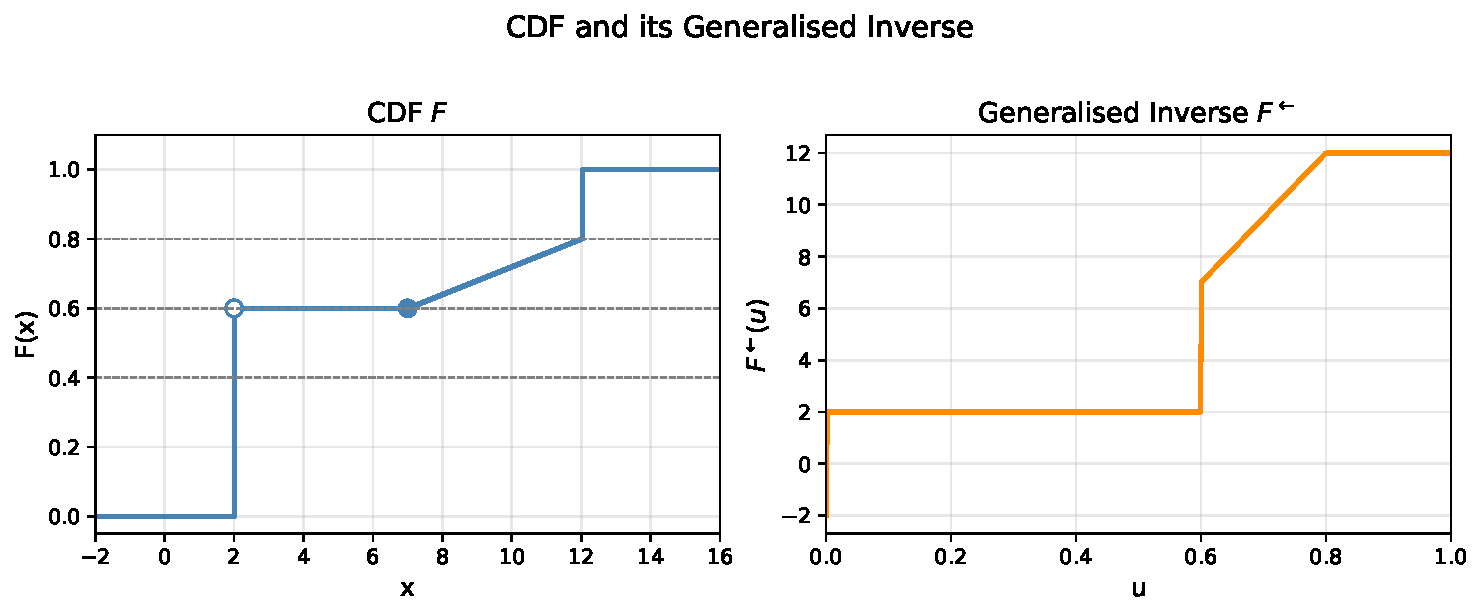
\includegraphics[width=0.78\textwidth]{fig_generalized_inverse}
  \caption{A c.d.f.\ $F$ with a flat region (left figure, shown by a dashed horizontal
    line at level $u_1$) creates a jump in $\FInv$: several values of $u$ all map to
    the same quantile.  Conversely, a jump in $F$ (a vertical step, right figure)
    creates a flat region in $\FInv$: a whole interval of quantile levels maps to
    the same $x$ value.  The point $x_1 = \FInv(u_1)$ is the leftmost $x$ with
    $F(x) \ge u_1$.}
\end{figure}

\end{frame}

\begin{frame}[allowframebreaks]{3.1 The ITM Theorem and Algorithm}

We now state and prove the central result that justifies the entire method.
The theorem has two parts: part (a) says we can \emph{generate} a sample from $F$
using a single uniform, and part (b) says the inverse is also true --- applying $F$
to a sample from $F$ recovers a uniform.

\begin{block}{Proposition 3.1.2 --- The Inverse Transform Theorem}
  \begin{enumerate}[(a)]
    \item \textbf{Sampling direction:} If $U \sim \UU[0,1)$, then
          $X = \FInv(U)$ has distribution $F$, meaning $\PP(X \le x) = F(x)$
          for all $x \in \RR$.
    \item \textbf{Probability-integral transform:} If $F$ is continuous and
          $X \sim F$ (i.e.\ $X$ has c.d.f.\ $F$), then $F(X) \sim \UU[0,1)$.
  \end{enumerate}
\end{block}

\textbf{Proof of part (a) --- step by step.}
We want to show $\PP(\FInv(U) \le x) = F(x)$.  We apply Lemma 3.1.1,
which says $\FInv(U) \le x$ happens if and only if $U \le F(x)$:
\[
  \PP\!\bigl(\FInv(U) \le x\bigr)
  \;\overset{\text{Lemma 3.1.1}}{=}\;
  \PP\!\bigl(U \le F(x)\bigr)
  \;\overset{U \sim \UU[0,1)}{=}\;
  F(x).
\]
The last step uses the fact that $\PP(U \le t) = t$ for any $t \in [0,1]$
when $U$ is uniform on $[0,1)$.

\textbf{Proof of part (b).}  For any $u \in (0,1)$, by Property (P5),
$F(\FInv(u)) = u$ when $F$ is continuous.  Therefore:
\[
  \PP(F(X) \le u) = \PP(X \le \FInv(u)) = F(\FInv(u)) = u.
\]
Since $\PP(F(X) \le u) = u$ for all $u$, the variable $F(X)$ is $\UU[0,1)$.

\framebreak

\begin{alertblock}{Algorithm 6 --- ITM: Generate $X \sim F$}
  \textbf{Require:} A c.d.f.\ $F$, or an efficient algorithm for computing
  the generalized inverse $\FInv(u)$ for any $u \in (0,1)$. \\
  \textbf{Ensure:} The output $X$ has the distribution $F$.
  \begin{enumerate}
    \item Generate $U \sim \UU[0,1)$ (one uniform random number).
    \item Compute $X = \FInv(U)$.
    \item Return $X$.
  \end{enumerate}
\end{alertblock}

A useful variant: since $1 - U \sim \UU[0,1)$ whenever $U \sim \UU[0,1)$,
we can equivalently use $Y = \overline{F}^{\leftarrow}(U)$, where
$\overline{F}^{\leftarrow}(u) = \FInv(1 - u)$ is the quantile of the tail
function.  This variant is convenient for distributions like the exponential
where the tail function has a simpler closed-form inverse than $F$ itself.

\begin{alertblock}{Key Insight: ITM Reduces Sampling to Inversion}
  The ITM theorem tells us that sampling from \emph{any} distribution reduces
  to exactly two steps: (1) draw one uniform number, and (2) evaluate $\FInv$.
  The entire difficulty is therefore concentrated in step (2).
  For many distributions, $\FInv$ has a simple closed form (exponential, Pareto,
  geometric).  For the normal distribution, $\FInv = \Phi^{-1}$ has no closed
  form and must be approximated numerically.
\end{alertblock}

\textbf{Corollary 3.1.3 (Uniform $p$-values).}
If $T$ is a test statistic whose c.d.f.\ $F$ is continuous, then the
$p$-value $p = 1 - F(T) = \overline{F}(T)$ is exactly $\UU[0,1)$-distributed
under the null hypothesis.  This is the theoretical justification for the
second-level uniformity testing procedure of Chapter 2.

\end{frame}

\begin{frame}[allowframebreaks]{3.1 Worked Example: Exponential Distribution $\mathrm{Exp}(\lambda)$}

The exponential distribution is the canonical model for waiting times between
independent events --- for example, the time until the next customer arrives,
or the lifetime of an electronic component.  Its c.d.f.\ is
\[
  F(x) = \begin{cases} 0 & x < 0, \\ 1 - e^{-\lambda x} & x \ge 0. \end{cases}
\]

\begin{block}{Notation: Exponential Distribution $\mathrm{Exp}(\lambda)$}
  \begin{itemize}
    \item $\lambda$ (lambda) $> 0$: the \emph{rate parameter}, measuring how
      frequently events occur.  A larger $\lambda$ means more frequent arrivals
      and hence shorter average waiting times.
    \item $e^{-\lambda x}$: the exponential function raised to $-\lambda x$.
      This factor decreases from 1 (at $x = 0$) toward 0 as $x$ grows, which
      is why the exponential distribution has ``light tails.''
    \item Mean: $\EE[X] = 1/\lambda$ (average waiting time).
    \item Variance: $\mathrm{Var}(X) = 1/\lambda^2$.
  \end{itemize}
\end{block}

To apply ITM we need $\overline{F}^{\leftarrow}$, the quantile of the tail
function.  Setting $\overline{F}(x) = u$, i.e.\ $e^{-\lambda x} = u$, and solving
for $x$ (take logarithm of both sides: $-\lambda x = \log u$, so $x = -\log(u)/\lambda$):
\[
  \overline{F}^{\leftarrow}(u) \;=\; -\frac{1}{\lambda}\log(u).
\]

\begin{alertblock}{How to Read $X = -\log(U)/\lambda$}
  When $U$ is close to 1 (most of the probability mass), $-\log(U)$ is close
  to 0, giving a small value of $X$ --- short waiting times are common.
  When $U$ is close to 0 (a rare event), $-\log(U)$ is large, giving a long
  waiting time $X$ --- long waits are rare but possible.
  The rate $\lambda$ simply scales the output: doubling $\lambda$ halves all
  waiting times, keeping the same shape but compressing the distribution.
\end{alertblock}

\begin{block}{Algorithm 7 (ITM-Exp): Generate $X \sim \mathrm{Exp}(\lambda)$}
  \begin{enumerate}
    \item Generate $U \sim \UU[0,1)$.
    \item Set $X = -\log(U)/\lambda$.
    \item Return $X$.
  \end{enumerate}
\end{block}

\framebreak

\begin{exampleblock}{Worked Numerical Example}
  Suppose $\lambda = 2$ (so the mean waiting time is $1/\lambda = 0.5$ time units).
  We draw $U = 0.3$.  Then:
  \[
    X = -\frac{\log(0.3)}{2} = -\frac{-1.204}{2} = \frac{1.204}{2} \approx 0.602.
  \]
  This particular draw gave a waiting time of about $0.602$, which is above the
  mean of $0.5$ --- but not unreasonably so.  Over many draws, the sample average
  will converge to $1/\lambda = 0.5$.

  Another draw, $U = 0.9$, gives $X = -\log(0.9)/2 \approx 0.053$, a short wait.
  A rare draw $U = 0.01$ gives $X = -\log(0.01)/2 = 4.605/2 \approx 2.30$, a
  very long wait.
\end{exampleblock}

\begin{columns}
  \column{0.50\textwidth}
  \begin{figure}
    \centering
    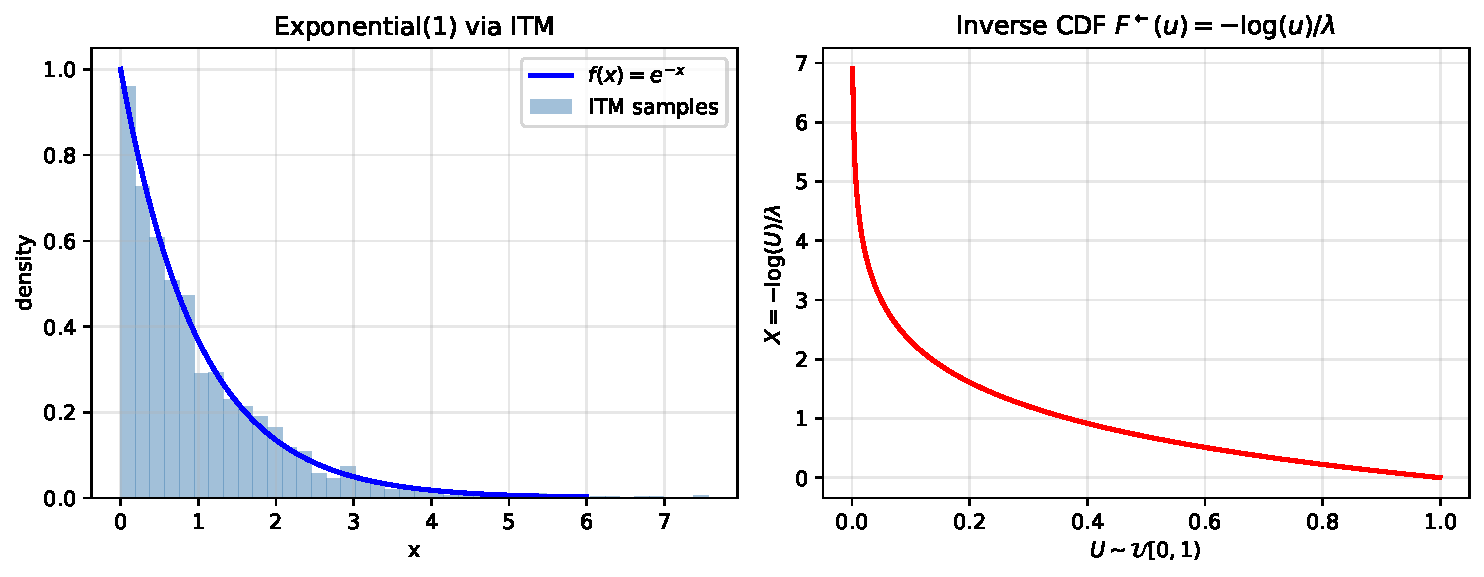
\includegraphics[width=\textwidth]{fig_itm_exponential}
    \caption{Histogram of $10\,000$ samples from $\mathrm{Exp}(2)$ generated via
      ITM (Algorithm 7).  The smooth curve is the true probability density
      $f(x) = 2e^{-2x}$.  The histogram closely tracks the theory.}
  \end{figure}
  \column{0.48\textwidth}
  \begin{figure}
    \centering
    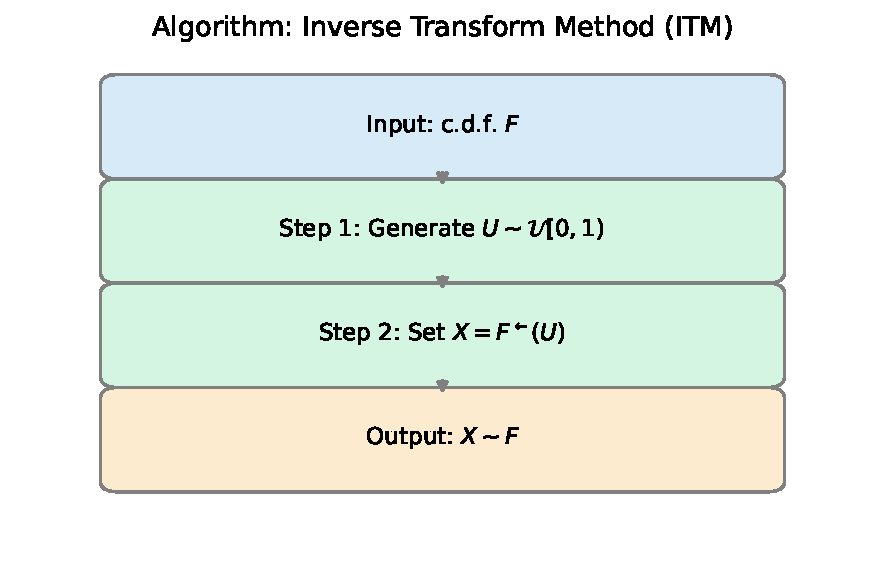
\includegraphics[width=\textwidth]{fig_itm_algorithm}
    \caption{Geometric picture of ITM: a uniform draw $U$ on the vertical axis
      (probability axis) is mapped horizontally to $X = F^{\leftarrow}(U)$ on
      the horizontal axis (value axis).  Regions where $F$ is steep (high density)
      produce many samples; flat regions (low density) produce few.}
  \end{figure}
\end{columns}

\end{frame}

\begin{frame}[allowframebreaks]{3.1 Worked Example: Pareto Distribution $\mathrm{Par}(\alpha)$}

The Pareto distribution is used to model phenomena where extreme values occur
with non-negligible probability.  Famous examples include the distribution of
wealth (a small fraction of people hold most of the wealth), the size of
insurance claims, and internet file sizes.  Its c.d.f.\ is
\[
  F(x) = \begin{cases} 0 & x < 0, \\ 1 - \dfrac{1}{(1+x)^{\alpha}} & x \ge 0. \end{cases}
\]

\begin{block}{Notation: Pareto Distribution $\mathrm{Par}(\alpha)$}
  \begin{itemize}
    \item $\alpha$ (alpha) $> 0$: the \emph{shape parameter} (also called
      the \emph{tail index}).  A \emph{smaller} $\alpha$ means a \emph{heavier}
      tail --- extreme values are more likely.
    \item $(1+x)^{-\alpha}$: this power-law decay is much slower than the
      exponential decay $e^{-\lambda x}$ of the exponential distribution, which
      is precisely why the Pareto has heavy tails.
    \item Mean: $\EE[X] = 1/(\alpha - 1)$ for $\alpha > 1$; the mean does
      \emph{not exist} (is infinite) for $\alpha \le 1$.
    \item Variance: finite only for $\alpha > 2$.
  \end{itemize}
\end{block}

To apply ITM, set $\overline{F}(x) = u$, i.e.\ $(1+x)^{-\alpha} = u$.
Raise both sides to the power $-1/\alpha$: $(1+x) = u^{-1/\alpha}$,
so $x = u^{-1/\alpha} - 1$.  Therefore $\overline{F}^{\leftarrow}(u) = u^{-1/\alpha} - 1$.

\begin{block}{Algorithm 8 (ITM-Par): Generate $X \sim \mathrm{Par}(\alpha)$}
  \begin{enumerate}
    \item Generate $U \sim \UU[0,1)$.
    \item Set $X = U^{-1/\alpha} - 1$.
    \item Return $X$.
  \end{enumerate}
\end{block}

\begin{exampleblock}{Worked Numerical Example}
  With $\alpha = 2$ (variance is infinite for $\alpha \le 2$, finite for $\alpha > 2$;
  this is the boundary case).  Draw $U = 0.5$:
  \[
    X = (0.5)^{-1/2} - 1 = \sqrt{2} - 1 \approx 0.414.
  \]
  Draw $U = 0.01$ (a rare small uniform value, representing a tail event):
  \[
    X = (0.01)^{-1/2} - 1 = 10 - 1 = 9.
  \]
  Notice how a small $U$ (probability 0.01) maps to a large $X = 9$,
  illustrating the heavy right tail.
\end{exampleblock}

\textbf{Two-parameter Pareto $\mathrm{Par}(\alpha, c)$.}
To create a family with a specified mean $m$ and tail index $\alpha$
(for $\alpha > 1$), set $c = (\alpha - 1)m$.  The c.d.f.\ is
$F(x) = 1 - c^\alpha/(c+x)^\alpha$ for $x \ge 0$.

\framebreak

\begin{columns}
  \column{0.52\textwidth}
  \begin{figure}
    \centering
    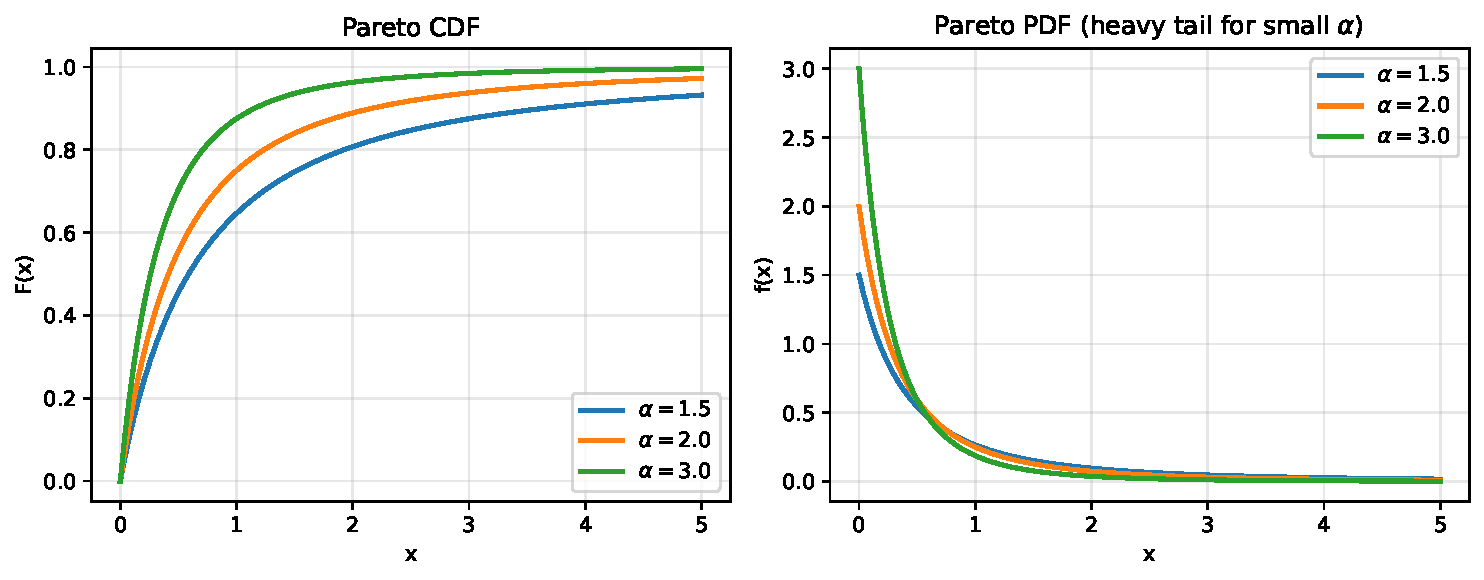
\includegraphics[width=\textwidth]{fig_pareto}
    \caption{Pareto c.d.f.\ (top) and p.d.f.\ (bottom) for $\alpha = 1.5$, $2$, and $3$.
      A smaller $\alpha$ (alpha) produces a heavier tail: the distribution assigns
      higher probability to very large values of $X$.  For $\alpha = 1.5$, the
      variance is infinite.}
  \end{figure}
  \column{0.46\textwidth}
  \begin{alertblock}{Key Insight: Light vs.\ Heavy Tails}
    For $\mathrm{Exp}(\lambda)$: all moments (mean, variance, etc.) are finite.
    Running averages of many samples converge smoothly to the true mean.

    \medskip
    For $\mathrm{Par}(\alpha)$: the $k$-th moment is finite only if $\alpha > k$.
    When $\alpha \le 2$, the variance is \emph{infinite}.  Running averages
    converge extremely slowly, and occasional enormous values cause dramatic
    spikes in the sample mean.

    \medskip
    Remarkably, the same ITM formula $X = U^{-1/\alpha} - 1$ works for any
    $\alpha > 0$, regardless of whether any moments are finite.
  \end{alertblock}
\end{columns}

\end{frame}

% ============================================================
\section{3.2 ITM Variants for Lattice Distributions}
% ============================================================

\begin{frame}[allowframebreaks]{3.2 ITM for Discrete (Lattice) Distributions}

Many quantities in practice take only integer values: the number of customers
in a queue, the number of defective items in a batch, the number of claims filed
in a day.  These are called \emph{lattice distributions}, where the random
variable $X$ takes values in $\{0, 1, 2, \ldots\}$ with probabilities
$p_k = \PP(X = k)$ for $k \ge 0$.  The function $(p_k)_{k \ge 0}$ is called
the \emph{probability mass function} (PMF).

The c.d.f.\ of a lattice distribution is a \emph{staircase function}:
$F(x) = \sum_{k=0}^{\lfloor x \rfloor} p_k$, which jumps by $p_k$ at each
integer $k$ and is constant between integers.  Its generalized inverse is:
$\FInv(u) = \min\{k : u \le F(k)\}$, the smallest integer $k$ such that the
cumulative probability $F(k)$ is at least $u$.

\begin{block}{Proposition 3.2.1 --- Discrete ITM}
  Let $U \sim \UU[0,1)$.  The random variable
  \[
    Y \;=\; \min\!\left\{k \ge 0 : U \le \sum_{i=0}^{k} p_i\right\}
  \]
  has probability mass function $(p_k)$.
\end{block}

\begin{block}{Notation for Proposition 3.2.1}
  \begin{itemize}
    \item $\sum_{i=0}^{k} p_i$ (Sigma, meaning ``sum''): the sum of probabilities
      $p_0 + p_1 + \cdots + p_k$, i.e.\ the cumulative probability $F(k)$.
    \item $\min\{\ldots\}$: the smallest element of the set, here the smallest
      non-negative integer satisfying the condition.
    \item The algorithm scans $k = 0, 1, 2, \ldots$ and stops at the first $k$
      for which the running total of probabilities reaches or exceeds $U$.
  \end{itemize}
\end{block}

\textbf{Proof.}  The event $\{Y = l\}$ occurs exactly when the cumulative
probability first crosses $U$ at step $l$, i.e.\ $F(l-1) < U \le F(l)$.
This interval has length $F(l) - F(l-1) = p_l$.  Since $U \sim \UU[0,1)$,
the probability of $U$ falling in any interval of length $p_l$ is exactly $p_l$.

\framebreak

\begin{alertblock}{Algorithm 9 (ITM-d): Generate $Y \sim (p_k)$}
  \textbf{Require:} The PMF $(p_k)_{k \ge 0}$ (all individual probabilities). \\
  \textbf{Ensure:} $Y$ follows the PMF $(p_k)$.
  \begin{enumerate}
    \item Set $Y \leftarrow 0$; generate $U \sim \UU[0,1)$; set $S \leftarrow p_0$.
    \item \textbf{While} $S < U$: increment $Y \leftarrow Y+1$, add $S \leftarrow S + p_Y$.
    \item Return $Y$.
  \end{enumerate}
  The variable $S$ accumulates the running sum of probabilities, and we stop
  when the sum first reaches or exceeds $U$.  The expected number of loop
  iterations equals $\EE[Y] + 1$, because on average we step through as many
  values as the expected output.  This means Algorithm 9 is slow for distributions
  with large expected values (large $\EE[Y]$).
\end{alertblock}

\textbf{Efficient recursion-based variant: Algorithm 10 (ITR).}
When the ratio $c_{k+1} = p_{k+1}/p_k$ has a simple closed form, we can avoid
storing the entire PMF and instead compute successive probabilities on the fly.
This is possible for the $(a,b,0)$ class of distributions, defined by the
recurrence $p_k = p_{k-1}(a + b/k)$ for constants $a$ and $b$.

\begin{block}{The $(a,b,0)$ Class and the ITR Algorithm}
  Three major count distributions belong to this class:
  \begin{itemize}
    \item \textbf{Binomial} $\mathrm{B}(n,p)$: $p_0 = (1-p)^n$,
          ratio $c_{k+1} = \dfrac{p(n-k)}{(1-p)(k+1)}$ for $k = 0,\ldots,n-1$.
          ($n$ = number of trials, $p$ = success probability.)
    \item \textbf{Poisson} $\mathrm{Poi}(\lambda)$: $p_0 = e^{-\lambda}$,
          ratio $c_{k+1} = \dfrac{\lambda}{k+1}$ for $k = 0,1,\ldots$
          ($\lambda$ (lambda) = rate parameter.)
    \item \textbf{Negative Binomial} $\mathrm{NB}(r,p)$: $p_0 = (1-p)^r$,
          ratio $c_{k+1} = \dfrac{(r+k)p}{k+1}$ for $k = 0,1,\ldots$
  \end{itemize}
\end{block}

\framebreak

\begin{alertblock}{Algorithm 10 (ITR): Generate $X \sim (p_k)$ via Ratio Recursion}
  \textbf{Require:} The starting probability $p_0$ and the ratios
  $c_{k+1} = p_{k+1}/p_k$ for $k = 0, 1, \ldots$
  \begin{enumerate}
    \item Set $S \leftarrow p_0$; $P \leftarrow p_0$; $X \leftarrow 0$.
    \item Generate $U \sim \UU[0,1)$.
    \item \textbf{While} $U > S$:
          set $X \leftarrow X+1$; $P \leftarrow P \cdot c_X$; $S \leftarrow S + P$.
    \item Return $X$.
  \end{enumerate}
  At each step, $P$ holds the current probability $p_X$, obtained by multiplying
  the previous probability by the ratio $c_X$.  This avoids pre-computing and
  storing the full PMF; we only ever hold two numbers ($S$ and $P$) in memory.
\end{alertblock}

\textbf{Special case: Geometric Distribution $\mathrm{Geo}(p)$.}
The geometric distribution models the number of failures before the first success,
with PMF $p_k = (1-p)^k \cdot p$ for $k = 0, 1, \ldots$ and mean $\EE[X] = (1-p)/p$.
Here $p$ is the success probability and $q = 1 - p$ is the failure probability.
For the geometric distribution, a closed-form inverse exists, bypassing the loop:
\[
  X = \lfloor \log U / \log(1-p) \rfloor \;\sim\; \mathrm{Geo}(p).
\]
\textbf{Proof.}  The survival function of $\mathrm{Geo}(p)$ is $\PP(X \ge k) = (1-p)^k$.
Setting $U \le (1-p)^k$ is equivalent to $\log U \le k \log(1-p)$ (since $\log(1-p) < 0$,
dividing reverses the inequality), giving $k \le \log U / \log(1-p)$.  The floor function
picks the largest such $k$.

\begin{figure}
  \centering
  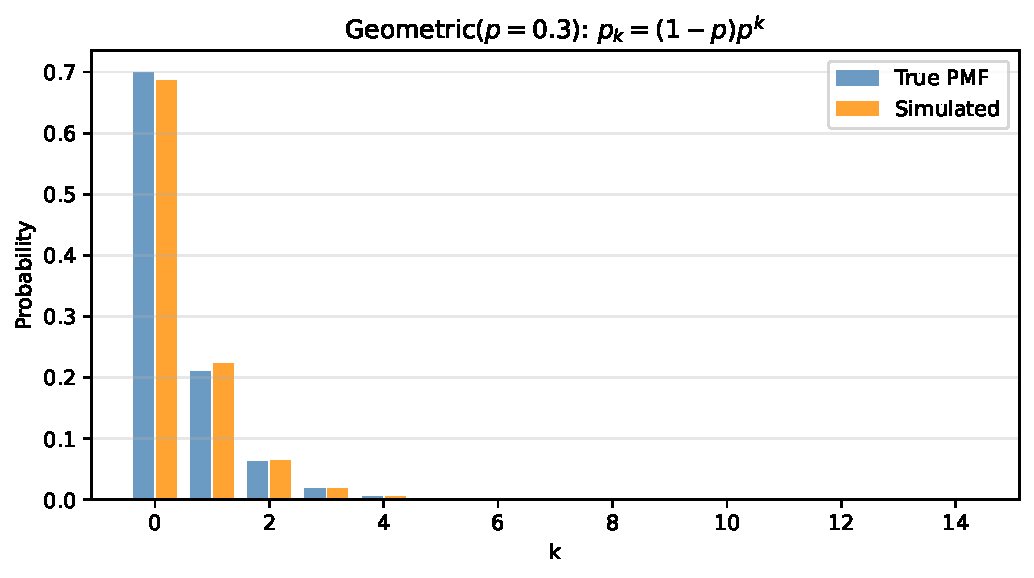
\includegraphics[width=0.45\textwidth]{fig_geometric}
  \caption{Histogram of $10\,000$ draws from $\mathrm{Geo}(p=0.3)$ via the closed-form
    ITM formula $X = \lfloor \log U / \log(0.7) \rfloor$, compared with the theoretical
    PMF (dots).  The match is excellent.}
\end{figure}

\end{frame}

% ============================================================
\section{3.3 Ad Hoc Methods}
% ============================================================

\begin{frame}[allowframebreaks]{3.3.1 Binomial Distribution $\mathrm{B}(n,p)$}

The binomial distribution models the total number of successes in $n$ independent
\emph{Bernoulli trials}, where each trial succeeds with probability $p$ and fails
with probability $1-p$.  The most natural simulation uses the defining structure
directly: generate each trial individually and count the successes.

Concretely, if we define $\xi_j = 1$ (success) or $\xi_j = 0$ (failure) for
trial $j$, then $X = \xi_1 + \xi_2 + \cdots + \xi_n$ counts the total successes.
Each $\xi_j$ can be simulated by drawing $U_j \sim \UU[0,1)$ and setting
$\xi_j = 1$ if $U_j \le p$, and $\xi_j = 0$ otherwise (since $\PP(U_j \le p) = p$).

\begin{alertblock}{Algorithm 11 (DB): Generate $X \sim \mathrm{B}(n,p)$}
  \textbf{Require:} Success probability $p \in (0,1)$ and number of trials $n \ge 1$.
  \begin{enumerate}
    \item Set $X \leftarrow 0$.
    \item For $i = 1$ to $n$:
    \begin{itemize}
      \item Generate $U \sim \UU[0,1)$.
      \item If $U \le p$: set $X \leftarrow X + 1$ (record a success).
    \end{itemize}
    \item Return $X$.
  \end{enumerate}
  This algorithm uses exactly $n$ uniform random numbers and performs $n$
  comparisons.  The expected output is $\EE[X] = np$ and the variance is
  $\mathrm{Var}(X) = np(1-p)$.  For large $n$ with moderate mean
  $\lambda = np$, the ITR algorithm (Algorithm 10) is asymptotically faster,
  since its expected cost is $O(\lambda)$ rather than $O(n)$.
\end{alertblock}

\begin{exampleblock}{Worked Numerical Example}
  Let $n = 5$ and $p = 0.4$.  Draw five uniforms:
  $U_1 = 0.72$, $U_2 = 0.15$, $U_3 = 0.63$, $U_4 = 0.38$, $U_5 = 0.81$.

  Compare each to the threshold $p = 0.4$:
  \begin{itemize}
    \item $U_1 = 0.72 > 0.4$: failure.
    \item $U_2 = 0.15 \le 0.4$: \textbf{success} ($X$ becomes 1).
    \item $U_3 = 0.63 > 0.4$: failure.
    \item $U_4 = 0.38 \le 0.4$: \textbf{success} ($X$ becomes 2).
    \item $U_5 = 0.81 > 0.4$: failure.
  \end{itemize}
  Result: $X = 2$.  The theoretical mean is $np = 5 \times 0.4 = 2.0$, so
  this particular draw returned exactly the mean.
\end{exampleblock}

\end{frame}

\begin{frame}[allowframebreaks]{3.3.2 Erlang Distribution $\mathrm{Erl}(n,\lambda)$}

The Erlang distribution models the total waiting time until the $n$-th event
in a Poisson process with rate $\lambda$.  For example, if customers arrive at
rate $\lambda = 3$ per minute, the time until the 5th customer arrives follows
$\mathrm{Erl}(5, 3)$.  Since each inter-arrival time is independently
$\mathrm{Exp}(\lambda)$, the Erlang distribution is simply the sum of $n$
independent exponentials.

\begin{block}{Definition and Simulation of $\mathrm{Erl}(n,\lambda)$}
  Let $Y_1, Y_2, \ldots, Y_n$ be independent, each $\sim \mathrm{Exp}(\lambda)$.
  Then the sum $X = Y_1 + Y_2 + \cdots + Y_n$ has the Erlang distribution
  $\mathrm{Erl}(n, \lambda)$.

  Using the ITM formula $Y_i = -\log(U_i)/\lambda$ for each exponential, and
  the logarithm property $\log(ab) = \log a + \log b$, we get the formula:
  \[
    X \;=\; -\frac{1}{\lambda}\!\left(\log U_1 + \log U_2 + \cdots + \log U_n\right)
       \;=\; -\frac{\log(U_1 \cdot U_2 \cdots U_n)}{\lambda},
  \]
  where $U_1, \ldots, U_n$ are independent $\UU[0,1)$ random variables.
\end{block}

\begin{block}{Notation for the Erlang Simulation Formula}
  \begin{itemize}
    \item $n$: the number of exponential stages (a positive integer).
    \item $\lambda$ (lambda) $> 0$: the rate of each exponential stage.
    \item $\log(\cdot)$: the natural logarithm (base $e \approx 2.718$).
    \item $U_1 \cdot U_2 \cdots U_n$: the product of all $n$ uniform draws.
      This product lies in $(0,1)$, so its logarithm is negative, and the
      negative sign at the front makes $X$ positive.
    \item Mean: $\EE[X] = n/\lambda$; Variance: $\mathrm{Var}(X) = n/\lambda^2$.
  \end{itemize}
\end{block}

\textbf{Important numerical note.}  When $n$ is large, computing the product
$U_1 \cdots U_n$ directly risks \emph{underflow}: with 64-bit floating-point
numbers, the product of 1000 values each around 0.5 underflows to zero.
Always accumulate the \emph{sum of logarithms}
$\log U_1 + \log U_2 + \cdots + \log U_n$ instead.

\framebreak

The survival function of $\mathrm{Erl}(n,\lambda)$ has an elegant closed-form
expression that we will use in the next section to derive a Poisson sampler:
\[
  \overline{F}(x) = \PP(X > x) = e^{-\lambda x}\!\left(1 + \lambda x + \frac{(\lambda x)^2}{2!}
    + \cdots + \frac{(\lambda x)^{n-1}}{(n-1)!}\right).
\]
This is a partial sum of the Taylor series of $e^{\lambda x}$, multiplied by
$e^{-\lambda x}$.

The probability density function of $\mathrm{Erl}(n,\lambda)$ is
$f(x) = \frac{\lambda^n}{\Gamma(n)} x^{n-1} e^{-\lambda x}$ for $x \ge 0$,
where $\Gamma(n) = (n-1)!$ for integer $n$.  This is a special case of the
Gamma distribution $\mathrm{Gamma}(n, \lambda)$.

\begin{figure}
  \centering
  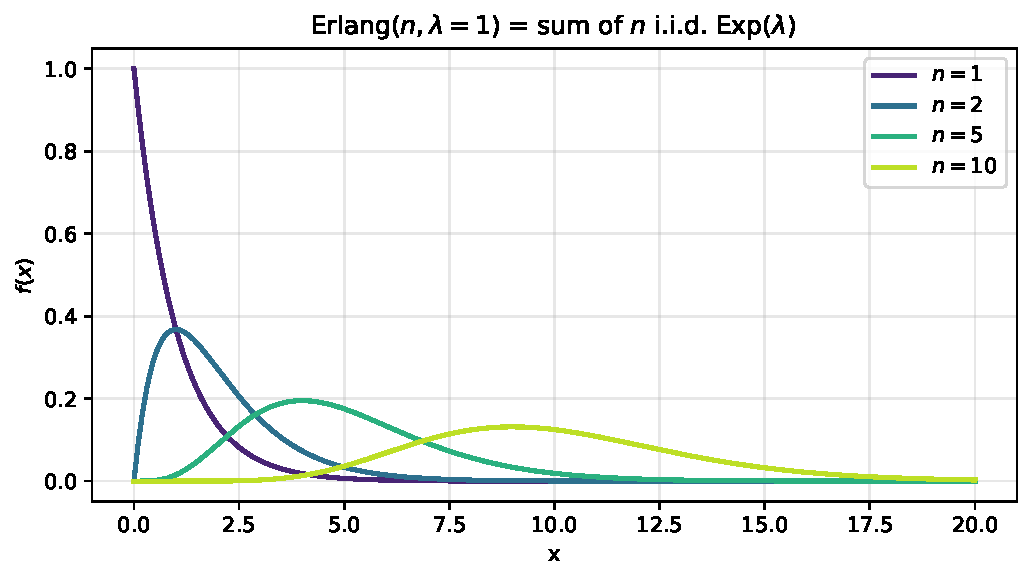
\includegraphics[width=0.50\textwidth]{fig_erlang}
  \caption{Erlang densities for $\mathrm{Erl}(n, 1)$ with $n = 1, 2, 3, 5$.
    When $n = 1$ the Erlang is simply $\mathrm{Exp}(1)$ (exponential).
    As $n$ increases, the distribution becomes more symmetric and concentrates
    closer to its mean $n/\lambda = n$, reflecting the averaging effect of
    summing many independent exponentials.}
\end{figure}

\end{frame}

\begin{frame}[allowframebreaks]{3.3.3 Poisson Distribution $\mathrm{Poi}(\lambda)$}

The Poisson distribution counts the number of events that occur in a fixed
time window $[0,1]$ when events arrive at rate $\lambda > 0$ independently
of each other.  We derive a beautiful simulation algorithm from the
\emph{renewal process} interpretation of the Poisson process.

\textbf{Idea.}  Imagine inter-arrival times $\tau_1, \tau_2, \ldots$ each
drawn independently from $\mathrm{Exp}(1)$, representing the gaps between
successive events.  The partial sum $\sigma_k = \tau_1 + \tau_2 + \cdots + \tau_k$
is the time of the $k$-th event.  The number of events in the window $(0, \lambda]$
is:
\[
  N = \begin{cases}
    \max\{i \ge 1 : \tau_1 + \cdots + \tau_i \le \lambda\} & \text{if } \tau_1 \le \lambda, \\
    0 & \text{if } \tau_1 > \lambda.
  \end{cases}
\]

\begin{block}{Proposition 3.3.1 --- Poisson via Renewal Process}
  $N$ (defined above) has the Poisson distribution: $N \sim \mathrm{Poi}(\lambda)$.
\end{block}

\textbf{Proof sketch.}  Using the Erlang survival formula from the previous slide:
$\PP(N \le k) = \PP(\sigma_{k+1} > \lambda) = e^{-\lambda}(1 + \lambda + \cdots + \lambda^k/k!)$.
The PMF then follows:
\[
  \PP(N = k) = \PP(N \le k) - \PP(N \le k-1)
    = e^{-\lambda}\frac{\lambda^k}{k!},
\]
which is exactly the Poisson PMF.

\framebreak

Substituting $\tau_i = -\log U_i$ (the ITM formula for $\mathrm{Exp}(1)$)
transforms the stopping criterion $\sum_{i=1}^n \tau_i \le \lambda$ into an
equivalent criterion about products:
\[
  \tau_1 + \cdots + \tau_n \le \lambda
  \;\iff\;
  -(\log U_1 + \cdots + \log U_n) \le \lambda
  \;\iff\;
  \log(U_1 \cdots U_n) \ge -\lambda
  \;\iff\;
  \prod_{i=1}^{n} U_i \ge e^{-\lambda}.
\]
So we count how many uniform numbers we can multiply before the running product
falls below $e^{-\lambda}$ (lambda = rate parameter).

\begin{alertblock}{Algorithm 12 (DP): Generate $X \sim \mathrm{Poi}(\lambda)$}
  \textbf{Require:} Rate parameter $\lambda > 0$.
  \begin{enumerate}
    \item Set $X \leftarrow 0$; generate $U \sim \UU[0,1)$; set $S \leftarrow -\log U$.
    \item \textbf{While} $S < \lambda$:
    \begin{itemize}
      \item Generate $U \sim \UU[0,1)$; set $S \leftarrow S - \log U$; set $X \leftarrow X + 1$.
    \end{itemize}
    \item Return $X$.
  \end{enumerate}
  The variable $S$ accumulates the sum $-\log U_1 - \log U_2 - \cdots$, which
  equals $\tau_1 + \tau_2 + \cdots$ (a sum of $\mathrm{Exp}(1)$ inter-arrivals).
  We stop when the total time first exceeds $\lambda$.
  The expected number of uniform random numbers consumed is $\EE[X] + 1 = \lambda + 1$.
\end{alertblock}

\begin{exampleblock}{Worked Numerical Example}
  Let $\lambda = 2$.  Draw $U_1 = 0.7$, $U_2 = 0.5$, $U_3 = 0.3$.
  \begin{enumerate}
    \item $S = -\log(0.7) \approx 0.357$.  Is $S < 2$?  Yes.  $X = 1$.
    \item $S = 0.357 + (-\log(0.5)) = 0.357 + 0.693 = 1.050$.  Is $S < 2$?  Yes.  $X = 2$.
    \item $S = 1.050 + (-\log(0.3)) = 1.050 + 1.204 = 2.254$.  Is $S < 2$?  No.  Stop.
  \end{enumerate}
  Result: $X = 2$.  The theoretical mean is $\lambda = 2$.
\end{exampleblock}

\framebreak

\begin{columns}
  \column{0.50\textwidth}
  \begin{figure}
    \centering
    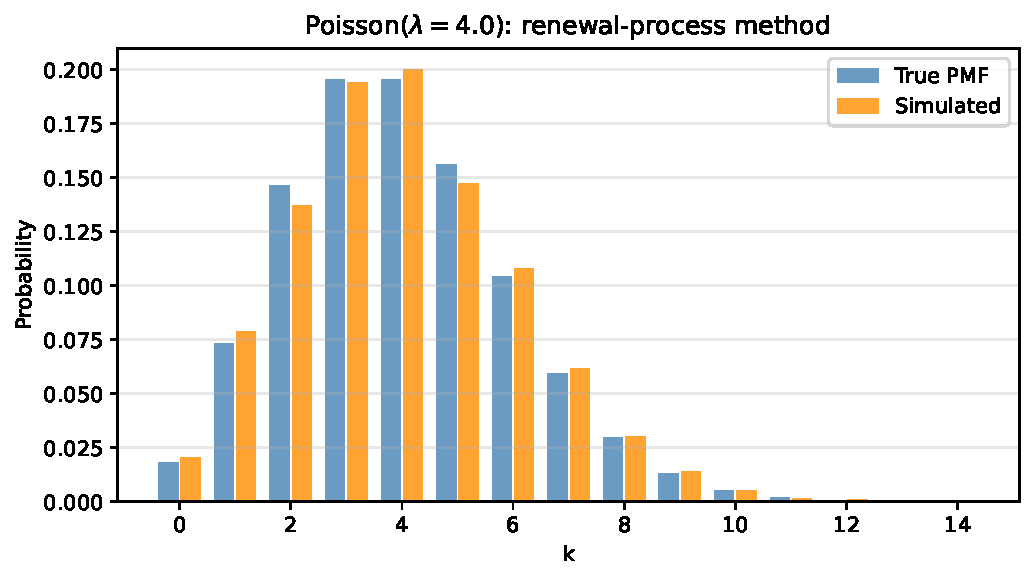
\includegraphics[width=\textwidth]{fig_poisson}
    \caption{Histogram of $10\,000$ samples from $\mathrm{Poi}(3)$ generated
      via Algorithm 12 (DP), compared with the true PMF (dots).  The
      empirical frequencies closely match the theoretical probabilities.}
  \end{figure}
  \column{0.48\textwidth}
  \begin{alertblock}{Key Insight: Poisson as a Counting Problem}
    Algorithm 12 gives a beautiful probabilistic interpretation: we are
    watching a Poisson process unfold in real time.  Each $-\log U_i$ is
    an $\mathrm{Exp}(1)$ inter-arrival time.  We count how many arrivals
    ($X$ events) fit before the total elapsed time $S$ exceeds the
    window length $\lambda$.  This connects simulation directly to the
    underlying physical model of the Poisson process.
  \end{alertblock}
\end{columns}

\end{frame}

\begin{frame}[fragile]{3.3 Python: Poisson and Erlang Simulation}
\begin{lstlisting}[style=python, caption={Ad hoc methods for Poisson and Erlang distributions (Algorithms 12 and Erlang sum)}]
import numpy as np
rng = np.random.default_rng(0)

def sample_poisson(lam, rng):
    """Renewal-process algorithm (Alg. 12) for Poi(lam).
    Accumulate Exp(1) inter-arrivals until total exceeds lam."""
    U = rng.uniform()
    S = -np.log(U)   # first Exp(1) inter-arrival time
    X = 0
    while S < lam:
        U = rng.uniform()
        S -= np.log(U)   # add next Exp(1) inter-arrival
        X += 1
    return X

def sample_erlang(n, lam, rng):
    """Sum of n Exp(lam) variables => Erl(n, lam).
    Numerically stable: accumulate logs, never multiply."""
    logs = rng.uniform(0, 1, n)
    return -np.log(logs).sum() / lam

# Verify: empirical vs theoretical moments
samples_poi = [sample_poisson(3.5, rng) for _ in range(10000)]
samples_erl = [sample_erlang(4, 1.0, rng) for _ in range(10000)]
print(f"Poi(3.5) mean = {np.mean(samples_poi):.3f}  (theory: 3.5)")
print(f"Erl(4,1) mean = {np.mean(samples_erl):.3f}  (theory: 4.0)")
print(f"Erl(4,1) var  = {np.var(samples_erl):.3f}   (theory: 4.0)")
\end{lstlisting}
\end{frame}

% ============================================================
\section{3.4 Uniform Distribution on Geometric Shapes}
% ============================================================

\begin{frame}[allowframebreaks]{3.4 Uniform Distribution on Subsets of $\RR^d$}

A random vector $\mathbf{X} \in A \subset \RR^d$ has the \emph{uniform distribution}
$\UU(A)$ if it is equally likely to fall anywhere in $A$.  Formally, for any
measurable subset $D \subset A$,
\[
  \PP(\mathbf{X} \in D) = \frac{\Vol D}{\Vol A},
\]
where $\Vol$ denotes the $d$-dimensional volume (length for $d=1$, area for $d=2$,
ordinary volume for $d=3$).  Equivalently, the density is
$f(\mathbf{x}) = \frac{1}{\Vol A}\mathbf{1}(\mathbf{x} \in A)$,
where $\mathbf{1}(\cdot)$ is the indicator function (1 if $\mathbf{x} \in A$, else 0).

\textbf{Rectangular regions.}  Sampling uniformly in the rectangle
$[a_1,b_1] \times \cdots \times [a_d,b_d]$ is straightforward:
generate $d$ independent uniforms $U_1, \ldots, U_d \sim \UU[0,1)$ and apply
a linear rescaling: $V_i = (b_i - a_i)U_i + a_i$ for $i = 1, \ldots, d$.
The output $\mathbf{V} = (V_1, \ldots, V_d)$ is then uniform in the rectangle.

For non-rectangular regions, a rejection approach based on the following
proposition works well in low dimensions.

\begin{block}{Proposition 3.4.1 --- Uniform on a Subset via Rejection}
  Let $A \subset B$ be measurable sets with $\Vol(B) < \infty$.
  If $\mathbf{X} \sim \UU(B)$ (uniform in the larger set $B$), then the
  conditional distribution $(\mathbf{X} \mid \mathbf{X} \in A)$ is $\UU(A)$.
\end{block}

\textbf{Proof.}  For any $D \subset A$, by the definition of conditional probability:
\[
  \PP(\mathbf{X} \in D \mid \mathbf{X} \in A)
  = \frac{\PP(\mathbf{X} \in D)}{\PP(\mathbf{X} \in A)}
  = \frac{\Vol D / \Vol B}{\Vol A / \Vol B}
  = \frac{\Vol D}{\Vol A}.
\]
This is the uniform distribution on $A$.

\framebreak

\begin{alertblock}{Algorithm 13 --- Rejection Sampling for $\UU(A)$}
  \textbf{Require:} A bounding rectangle $B = [a_1,b_1] \times \cdots \times [a_d,b_d]$
  containing $A$, and a way to test whether a point $\mathbf{V}$ lies in $A$.
  \begin{enumerate}
    \item Generate $U_1, \ldots, U_d$ i.i.d.\ $\UU[0,1)$; set
          $V_i = (b_i - a_i)U_i + a_i$ for each $i = 1, \ldots, d$.
    \item If $\mathbf{V} = (V_1, \ldots, V_d) \in A$: set $\mathbf{X} = \mathbf{V}$
          and return $\mathbf{X}$.
    \item Otherwise go back to step 1 and try again.
  \end{enumerate}
  Each trial is accepted with probability $\Vol(A)/\Vol(B)$.
  The expected number of trials is $\Vol(B)/\Vol(A)$.
\end{alertblock}

\textbf{The curse of dimensionality for $d$-dimensional balls.}
The $d$-dimensional unit ball $B_d = \{\mathbf{x} \in \RR^d : \|\mathbf{x}\| \le 1\}$
has volume $\Vol(B_d) = \pi^{d/2}/\Gamma(d/2+1)$, where $\Gamma$ (Gamma) is
the generalization of the factorial function.  The enclosing hypercube
$[-1,1]^d$ has volume $2^d$.  Their ratio is:
\[
  \frac{\Vol(B_d)}{\Vol([-1,1]^d)} = \frac{\pi^{d/2}}{2^d\,\Gamma(d/2+1)}
  \;\xrightarrow{d \to \infty}\; 0
\]
exponentially fast.

\begin{alertblock}{How Bad Is the Curse?}
  At $d = 2$: acceptance probability $= \pi/4 \approx 78.5\%$ (quite good).
  At $d = 10$: acceptance probability $\approx 0.25\%$ (1 in 400).
  At $d = 30$: acceptance probability $\approx 2 \times 10^{-14}$ (1 in $5 \times 10^{13}$).
  Algorithm 13 is therefore completely impractical for high-dimensional balls.
  Section 3.8 provides the correct approach using the Normal distribution trick.
\end{alertblock}

\end{frame}

% ============================================================
\section{3.5 Acceptance-Rejection Method}
% ============================================================

\begin{frame}[allowframebreaks]{3.5.1 AR-d: Discrete Acceptance-Rejection}

The acceptance-rejection (AR) method, introduced by John von Neumann, is the
most adaptable general-purpose sampling technique.  It applies whenever we want
to sample from a target distribution $(p_j)$ but can only easily sample from
a ``proposal'' distribution $(q_j)$.  The method requires a finite constant
$c \ge 1$ such that $p_j \le c \, q_j$ for every $j$ in the state space.

\textbf{Intuition.}  Think of $q_j$ as a budget of probability mass allocated
to value $j$.  The target $p_j$ is at most $c \, q_j$, so the ratio
$p_j/(c \, q_j) \in [0,1]$ measures what fraction of the budget at $j$ should
``count.''  We propose a value $Y = j$ from the easy distribution, then
accept it with probability $p_j/(c \, q_j)$.  If accepted, the output $X = j$
has the correct distribution $(p_j)$; if rejected, we try again.

\begin{block}{Proposition 3.5.1 --- AR-d Correctness}
  Let $U \sim \UU[0,1)$ and $Y \sim (q_j)$ be independent.
  Define the acceptance event $A = \{c \, U \, q_Y \le p_Y\}$.
  Then the acceptance probability and conditional distribution are:
  \[
    \PP(A) = \frac{1}{c} \qquad \text{and} \qquad \PP(Y = j \mid A) = p_j.
  \]
\end{block}

\begin{block}{Notation for Proposition 3.5.1}
  \begin{itemize}
    \item $c$: the \emph{bounding constant}, satisfying $\sup_j p_j/q_j \le c$.
      A smaller $c$ means higher acceptance probability $1/c$, so we want
      $c$ as small as possible.
    \item $A$: the event that the proposed value $Y$ is accepted.
      Acceptance happens when $U \le p_Y/(c \, q_Y)$, i.e.\ when the uniform
      draw falls below the ratio of the target probability to the proposal times $c$.
    \item $\PP(A) = 1/c$: on average, we need $c$ proposals per accepted sample.
  \end{itemize}
\end{block}

\textbf{Proof.}  By conditioning on the proposed value $Y = j$:
\[
  \PP(Y = j, A)
  = q_j \cdot \PP\!\left(U \le \frac{p_j}{c q_j}\right)
  = q_j \cdot \frac{p_j}{c q_j}
  = \frac{p_j}{c}.
\]
Summing over all $j$: $\PP(A) = \sum_j p_j/c = 1/c$.
Finally, $\PP(Y = j \mid A) = \PP(Y = j, A)/\PP(A) = (p_j/c)/(1/c) = p_j$.

\framebreak

\begin{alertblock}{Algorithm 14 (AR-d): Generate $X \sim (p_j)$}
  \textbf{Require:} Bounding constant $c$ with $p_j \le c q_j$ for all $j$;
  an algorithm for sampling $Y \sim (q_j)$.
  \begin{enumerate}
    \item \textbf{Repeat:}
    \begin{itemize}
      \item Generate $Y \sim (q_j)$ and independently $U \sim \UU[0,1)$.
    \end{itemize}
    \item \textbf{Until} $c \, U \, q_Y \le p_Y$ (acceptance test).
    \item Return $X = Y$.
  \end{enumerate}
  The number of loop iterations $L$ has a geometric distribution:
  $\PP(L = k) = (1 - 1/c)^{k-1} \cdot (1/c)$, with mean $\EE[L] = c$.
  A smaller $c$ means fewer iterations.  Therefore always choose the
  \emph{smallest} possible $c$, i.e.\ $c = \sup_j p_j/q_j$.
\end{alertblock}

\begin{exampleblock}{Example 3.5.2 --- Sampling from the Zeta Distribution}
  We want to sample $X$ with PMF $p_j = \frac{6}{\pi^2 j^2}$ for $j = 1, 2, \ldots$
  (proportional to $1/j^2$; normalised by $\sum_{j=1}^\infty 1/j^2 = \pi^2/6$).

  \textbf{Proposal:} $q_j = 1/(j(j+1))$ for $j = 1, 2, \ldots$  This is easy to sample:
  note $1/(j(j+1)) = 1/j - 1/(j+1)$, so $F_q(k) = 1 - 1/(k+1)$,
  and $Y = \lfloor 1/(1-U) \rfloor$ generates $Y \sim (q_j)$.

  \textbf{Bounding constant:} The ratio $p_j/q_j = \frac{6}{\pi^2 j^2} \cdot j(j+1)
  = \frac{6(j+1)}{\pi^2 j}$, which is maximized at $j = 1$ giving $c = 12/\pi^2 \approx 1.216$.

  \textbf{Acceptance condition:} $c U q_Y \le p_Y$ simplifies to $2UY \le Y + 1$.
  The acceptance rate is $1/c = \pi^2/12 \approx 82.2\%$.
\end{exampleblock}

\end{frame}

\begin{frame}[allowframebreaks]{3.5.2 AR-c: Continuous Acceptance-Rejection}

The continuous version of the AR method targets a continuous density $f(x)$
on a set $E \subseteq \RR^d$, using a proposal density $g(x)$.  The requirement
is the same: there must exist a finite constant $c$ such that $f(x) \le c \, g(x)$
for all $x \in E$.  This means the scaled proposal density $c \, g(x)$ forms an
\emph{envelope} above the target density everywhere.

\begin{block}{Proposition 3.5.3 --- AR-c Correctness}
  Let $Y \sim g$ and $U \sim \UU[0,1)$ be independent (that is, $Y$ is drawn
  from the proposal density $g$, and $U$ is an independent uniform).
  Define the acceptance event $A = \{c \, U \, g(Y) \le f(Y)\}$.
  Then the acceptance probability and the conditional distribution of $Y$ given
  acceptance are:
  \[
    \PP(A) = \frac{1}{c} \qquad \text{and} \qquad
    \PP(Y \in B \mid A) = \int_B f(y)\,dy \quad \text{for all } B \subset E.
  \]
\end{block}

\textbf{Proof.}  The joint density of $(U, Y)$ is $g(y)\,du\,dy$ on $[0,1] \times E$.
Restricting to the acceptance region $\{(u,y) : c \, u \, g(y) \le f(y)\}$:
\[
  \PP(Y \in B, A)
  = \int_B \int_0^{f(y)/(c\,g(y))} g(y)\,du\,dy
  = \int_B \frac{f(y)}{c}\,dy.
\]
Dividing by $\PP(A) = 1/c$ gives $\PP(Y \in B \mid A) = \int_B f(y)\,dy$.

\begin{alertblock}{Algorithm 16 (AR-c): Generate $X \sim f$}
  \textbf{Require:} Constant $c$ with $f(x) \le c \, g(x)$ for all $x$;
  an algorithm for sampling $Y \sim g$.
  \begin{enumerate}
    \item \textbf{Repeat:} generate $Y \sim g$ and independently $U \sim \UU[0,1)$.
    \item \textbf{Until} $c \, U \, g(Y) \le f(Y)$.
    \item Return $X = Y$.
  \end{enumerate}
\end{alertblock}

\framebreak

\textbf{Example 3.5.4 --- Generating $\NN(0,1)$ via AR-c (Algorithm AR-N).}

The standard normal density is $\phi(x) = \frac{1}{\sqrt{2\pi}} e^{-x^2/2}$
(phi, the Greek letter).  By symmetry, we first generate the absolute value
$|Z|$ from the \emph{half-normal} density
$f(x) = \frac{2}{\sqrt{2\pi}} e^{-x^2/2}$ for $x > 0$, then randomly negate it.

We use the $\mathrm{Exp}(1)$ density $g(x) = e^{-x}$ as the proposal, because
it is easy to sample via ITM and has a shape similar to $f$ on $(0,\infty)$.

The ratio $f(x)/g(x) = \frac{2}{\sqrt{2\pi}} e^{x - x^2/2}$.  To find the
bounding constant, maximize the exponent $h(x) = x - x^2/2$: set $h'(x) = 1 - x = 0$,
giving $x^* = 1$, $h(1) = 1/2$.  Therefore:
\[
  c = \frac{2}{\sqrt{2\pi}} e^{1/2} = \sqrt{\frac{2e}{\pi}} \approx 1.315.
\]
The acceptance rate is $1/c = \sqrt{\pi/(2e)} \approx 76.0\%$.

The acceptance condition $c U g(Y) \le f(Y)$ simplifies (dividing both sides
by $g(Y) = e^{-Y}$) to:
\[
  U \;\le\; \exp\!\left(-\frac{(Y-1)^2}{2}\right).
\]

\begin{block}{Algorithm 17 (AR-N): Generate $Z \sim \NN(0,1)$}
  \begin{enumerate}
    \item Generate $U_1 \sim \UU[0,1)$; set $Y = -\log(U_1)$.
          (This gives $Y \sim \mathrm{Exp}(1)$ via ITM.)
    \item Generate $U_2 \sim \UU[0,1)$ independently.
    \item If $U_2 > \exp(-(Y-1)^2/2)$: the proposal is rejected; go back to step 1.
    \item Generate $U_3 \sim \UU[0,1)$; set $I = 2\lfloor 2U_3\rfloor - 1$
          (so $I = +1$ or $I = -1$ with equal probability $1/2$).
    \item Return $Z = I \cdot Y$.
  \end{enumerate}
\end{block}

\begin{figure}
  \centering
  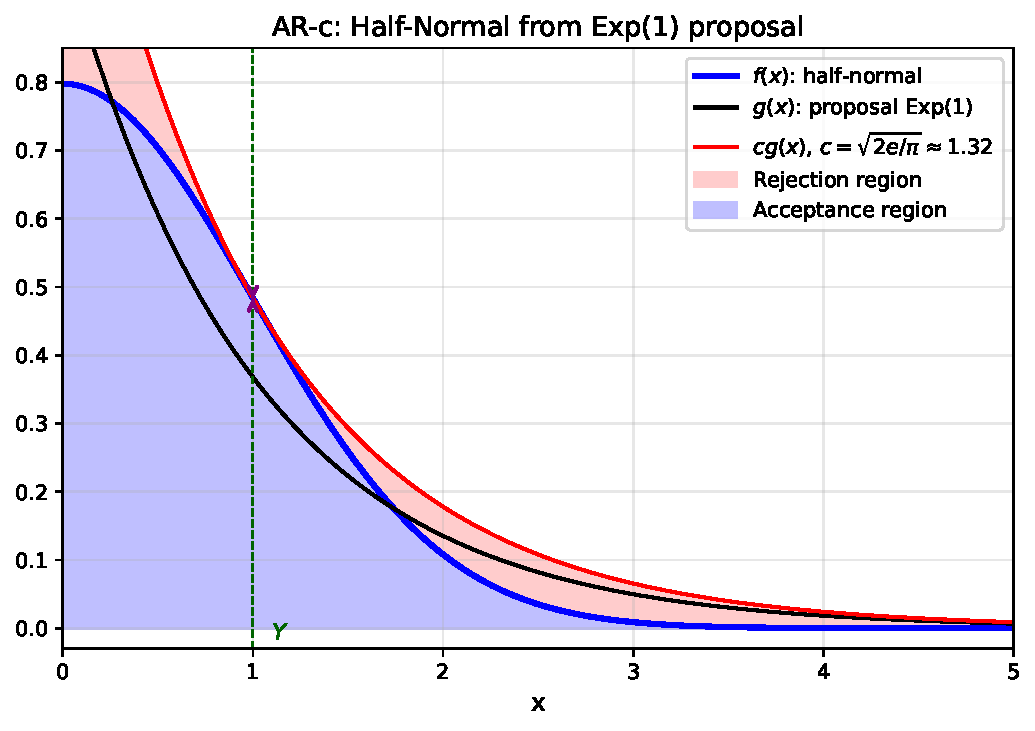
\includegraphics[width=0.55\textwidth]{fig_ar_halfnormal}
  \caption{The half-normal target density $f(x) = \sqrt{2/\pi}\,e^{-x^2/2}$ (blue),
    the proposal density $g(x) = e^{-x}$ of $\mathrm{Exp}(1)$ (gray), and the
    envelope $c \cdot g(x)$ (dashed orange).  A proposed point $(Y, U \cdot c \cdot g(Y))$
    is accepted when it falls in the blue region, i.e.\ below the target density $f$.}
\end{figure}

\framebreak

\textbf{Unknown normalising constants.}
In many practical settings (e.g.\ Bayesian inference), we only know the
unnormalised densities $f^*(x)$ and $g^*(x)$, related to the actual densities by
$f(x) = f^*(x)/c_f$ and $g(x) = g^*(x)/c_g$ for unknown constants $c_f$ and $c_g$.
In this case, compute $c^* = \sup_x f^*(x)/g^*(x)$.  The acceptance condition
$c U g(Y) \le f(Y)$ then becomes $c^* U g^*(Y) \le f^*(Y)$, which does not
require knowing $c_f$ or $c_g$.  This makes AR-c especially powerful for
Bayesian posterior sampling.

\textbf{Example 3.5.5 --- Gamma($\alpha$, $\lambda$) for $\alpha$ (alpha) $< 1$ (Madras).}
When $\alpha < 1$, the Gamma density $f(x) \propto x^{\alpha-1} e^{-\lambda x}$
is unbounded near $x = 0$.  The Madras algorithm uses a two-component mixture
proposal: a power-law density $g_1(x) \propto x^{\alpha-1}$ on $(0,1)$, and an
exponential density $g_2(x) = e^{-x}$ on $[1,\infty)$.  The bounding constant
is $c = 1/(K\,\Gamma(\alpha))$ where $K = \alpha e/(\alpha + e)$.

\textbf{Example 3.5.6 --- Central $\chi^2_d$ Distribution.}
The chi-squared distribution with $d$ degrees of freedom is $\chi^2_d = Z_1^2 + \cdots + Z_d^2$,
the sum of $d$ squared standard normals.  Since $\chi^2_d \sim \mathrm{Gamma}(d/2, 1/2)$,
and for even $d = 2k$ the Erlang formula applies: $\chi^2_{2k} \sim \mathrm{Erl}(k, 1/2)$,
which can be generated directly.

\end{frame}

\begin{frame}[fragile]{3.5 Python: AR-c for $\NN(0,1)$}
\begin{lstlisting}[style=python, caption={AR-N (Algorithm 17): generate standard normal via acceptance-rejection with Exp(1) proposal}]
import numpy as np
rng = np.random.default_rng(42)

def sample_normal_arn(n, rng):
    """
    Algorithm 17 AR-N: generate N(0,1) via AR-c.
    Target: half-normal f(x) = sqrt(2/pi)*exp(-x^2/2), x>0.
    Proposal: Exp(1), g(x) = exp(-x), x>0.
    Bounding constant c = sqrt(2e/pi) ~ 1.315.
    Acceptance rate: 1/c = sqrt(pi/(2e)) ~ 76.0%.
    """
    out = np.empty(n)
    i = 0
    total_trials = 0
    while i < n:
        U1 = rng.uniform()
        Y  = -np.log(U1)               # Y ~ Exp(1) via ITM
        U2 = rng.uniform()
        total_trials += 1
        if U2 <= np.exp(-(Y - 1)**2 / 2):   # acceptance test
            sign = 1 if rng.uniform() < 0.5 else -1
            out[i] = sign * Y
            i += 1
    print(f"Acceptance rate: {n/total_trials:.3f}  "
          f"(theory: {np.sqrt(np.pi/(2*np.e)):.3f})")
    return out

Z = sample_normal_arn(5000, rng)
print(f"Mean: {Z.mean():.4f}  (theory: 0)")
print(f"Std:  {Z.std():.4f}   (theory: 1)")
\end{lstlisting}
\end{frame}

% ============================================================
\section{3.6 Composition Method}
% ============================================================

\begin{frame}[allowframebreaks]{3.6 Composition (Mixture) Method}

The composition method addresses the case where the target distribution is a
\emph{mixture}: its density (or PMF) can be written as a weighted combination
(a convex combination) of simpler component densities that we can already sample
efficiently.  If we know the component proportions and can sample each component,
then sampling the mixture is essentially free.

\begin{block}{Composition Method: Setup and Algorithm}
  Suppose the target density has the mixture form
  \[
    f(x) = \sum_{j=1}^{n} p_j\, g_j(x),
  \]
  where:
  \begin{itemize}
    \item each $g_j$ is a valid probability density function (non-negative,
      integrates to 1),
    \item $(p_j)_{j=1}^n$ is a probability vector: $p_j \ge 0$ and $\sum_j p_j = 1$,
    \item we can sample from each component density $g_j$ efficiently.
  \end{itemize}

  \textbf{Algorithm (Composition):}
  \begin{enumerate}
    \item Sample a component index $J$ with $\PP(J = j) = p_j$
          (this is itself a discrete sampling problem, solvable by ITM-d or a table).
    \item Conditional on $J = j$, sample $X \sim g_j$ from component $j$.
    \item Return $X$.
  \end{enumerate}

  The output $X$ has the mixture density $f$, because for any measurable set $B$:
  $\PP(X \in B) = \sum_j p_j \int_B g_j(x)\,dx = \int_B f(x)\,dx$.
\end{block}

\begin{alertblock}{How to Read the Composition Algorithm}
  Think of a mixture model as follows: there is a hidden ``type'' label $J$,
  and given $J = j$, the data comes from the $j$-th component.  The composition
  algorithm makes this generative story explicit: first pick the type $J$
  (with probability $p_j$), then sample from that type's distribution $g_j$.
  The marginal distribution of $X$ (ignoring $J$) is exactly the mixture $f$.
\end{alertblock}

The method extends naturally to \emph{infinite} mixtures:
$f(x) = \sum_{j=0}^{\infty} p_j g_j(x)$, where $J$ is now drawn from the
infinite PMF $(p_j)_{j \ge 0}$.

\framebreak

\begin{figure}
  \centering
  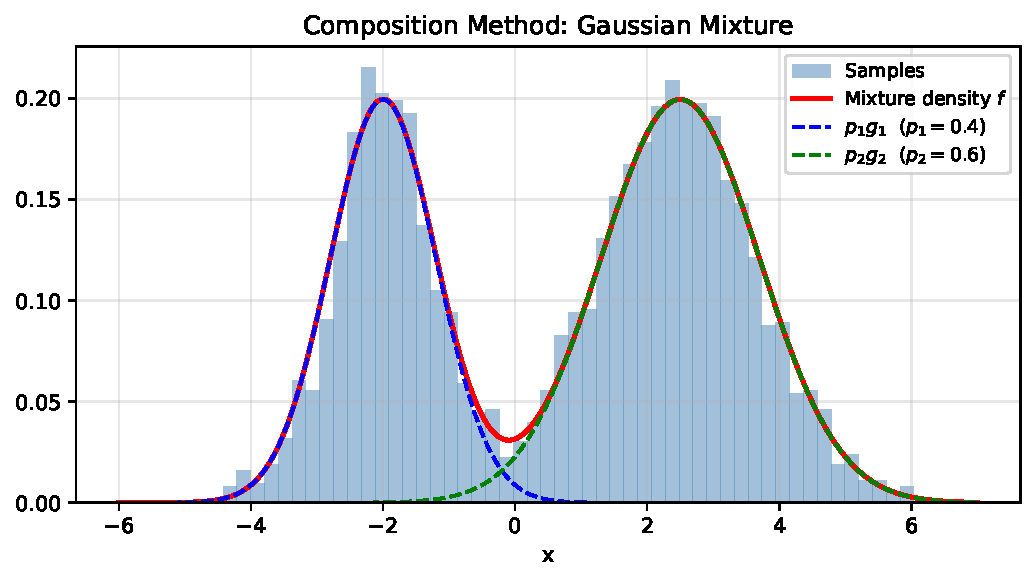
\includegraphics[width=0.55\textwidth]{fig_composition}
  \caption{A three-component Gaussian mixture
    $f = 0.3\,g_1 + 0.5\,g_2 + 0.2\,g_3$ (solid black curve) and its three
    component densities $g_1, g_2, g_3$ (dashed curves).  The composition
    method first samples $J \in \{1,2,3\}$ with probabilities $(0.3, 0.5, 0.2)$,
    then draws $X$ from component $g_J$.  The resulting samples are drawn from
    the bimodal mixture.}
\end{figure}

\textbf{Example 3.6.1 --- Non-central Chi-squared Distribution.}
The non-central chi-squared distribution with $d$ degrees of freedom and
non-centrality parameter $\lambda > 0$ (lambda) has a density that is an
infinite Poisson-weighted mixture of Gamma densities:
\[
  f(x) = \sum_{j=0}^{\infty} p_j(\lambda/2)\, g_j(x),
  \quad
  p_j(\mu) = \frac{\mu^j}{j!}e^{-\mu}, \quad g_j \sim \mathrm{Gamma}(j + d/2,\; 1/2).
\]
Here $\mu = \lambda/2$ (mu) is the Poisson rate for the mixture weight.  Simulation:
draw $J \sim \mathrm{Poi}(\lambda/2)$ (using Algorithm 12), then draw
$X \sim \mathrm{Gamma}(J + d/2, 1/2)$.

\framebreak

\textbf{Example 3.6.3 --- Gamma-Poisson Mixture (Negative Binomial).}
Suppose the rate $\Lambda$ (Lambda) of a Poisson process is itself random,
following a Gamma distribution: $\Lambda \sim \mathrm{Gamma}(\alpha, \lambda)$
with $\alpha$ (alpha) $> 0$ and $\lambda$ (lambda) $> 0$.  Conditional on
$\Lambda = \ell$, the count $X \sim \mathrm{Poi}(\ell)$.  The marginal
distribution of $X$ (averaging over the random rate) is:
\[
  p_n = \int_0^\infty \frac{\ell^n e^{-\ell}}{n!} \cdot
    \frac{\lambda^\alpha \ell^{\alpha-1} e^{-\lambda\ell}}{\Gamma(\alpha)}
    \,d\ell
  = \binom{n + \alpha - 1}{n}
    \!\left(\frac{1}{1+\lambda}\right)^{\!\alpha}
    \left(\frac{\lambda}{1+\lambda}\right)^{\!n},
\]
which is the Negative Binomial distribution $\mathrm{NB}(\alpha, 1/(1+\lambda))$.

\begin{alertblock}{Key Insight: Simulation via Hierarchical Models}
  The composition method is not just a computational trick --- it reveals the
  generative mechanism behind many distributions.  The Negative Binomial arises
  naturally from a Poisson process with a Gamma-distributed random rate.
  Simulating it via the hierarchy (draw $\Lambda$, then draw $X \mid \Lambda$)
  is both simple and interpretable.
\end{alertblock}

\end{frame}

\begin{frame}[fragile]{3.6 Python: Mixture Sampling}
\begin{lstlisting}[style=python, caption={Composition method for a Gaussian mixture and NB via Gamma-Poisson hierarchy}]
import numpy as np
rng = np.random.default_rng(0)

def sample_mixture(weights, mus, sigmas, n, rng):
    """
    Composition method for a Gaussian mixture.
    weights: mixture probabilities summing to 1.
    mus, sigmas: mean and std of each component.
    Step 1: sample component index J ~ Categorical(weights).
    Step 2: sample X from component J.
    """
    weights = np.array(weights)
    J = rng.choice(len(weights), size=n, p=weights)
    X = np.array([rng.normal(mus[j], sigmas[j]) for j in J])
    return X

def sample_nb_gamma_poisson(alpha, lam, n, rng):
    """
    Sample NB(alpha, 1/(1+lam)) via Gamma-Poisson hierarchy.
    Step 1: Lambda ~ Gamma(alpha, scale=1/lam).
    Step 2: X | Lambda ~ Poi(Lambda).
    """
    Lambda = rng.gamma(alpha, 1.0/lam, size=n)
    X = rng.poisson(Lambda)
    return X

# 3-component Gaussian mixture: weights, means, stds
w = [0.3, 0.5, 0.2];  mus = [-3., 1., 5.];  sigs = [0.8, 1.2, 0.5]
X = sample_mixture(w, mus, sigs, n=10000, rng=rng)
# Theoretical mean: 0.3*(-3) + 0.5*1 + 0.2*5 = -0.9+0.5+1.0 = 0.6
print(f"Mixture mean: {X.mean():.3f}  (theory: 0.600)")

Y = sample_nb_gamma_poisson(alpha=3.0, lam=2.0, n=10000, rng=rng)
# NB(3, 1/3) mean = alpha*(1-p)/p = 3*(2/3)/(1/3) = 6; or alpha/lam = 3/2
print(f"NB mean: {Y.mean():.3f}  (theory: {3.0/2.0:.3f})")
\end{lstlisting}
\end{frame}

% ============================================================
\section{3.7 Generating Gaussian Random Numbers}
% ============================================================

\begin{frame}[allowframebreaks]{3.7.1 Box-Muller Method}

The standard normal distribution $\NN(0,1)$ is the most important distribution
in statistics and simulation.  We present three methods for generating standard
normal samples; the first is the Box-Muller transform, which generates \emph{two}
independent $\NN(0,1)$ variables at once using polar coordinates.

The key structural observation is that the joint density of two independent
standard normals has a special factorization in polar coordinates.

\begin{block}{Lemma 3.7.1 --- Polar Structure of Bivariate Normal}
  Let $Z_1, Z_2 \stackrel{\text{i.i.d.}}{\sim} \NN(0,1)$ and let $(D, \Theta)$
  be their polar coordinates: $Z_1 = D\cos\Theta$, $Z_2 = D\sin\Theta$,
  where $D = \sqrt{Z_1^2 + Z_2^2}$ is the radius and $\Theta \in [0, 2\pi)$
  is the angle.  Then $D$ and $\Theta$ are \emph{independent}, with:
  \begin{itemize}
    \item $\Theta \sim \UU[0, 2\pi)$ (the angle is uniformly distributed).
    \item $D$ has the \textbf{Rayleigh} density $f_D(r) = r\,e^{-r^2/2}$ for $r > 0$.
  \end{itemize}
\end{block}

\textbf{Proof.}  The joint density of $(Z_1, Z_2)$ is
$f(z_1, z_2) = \frac{1}{2\pi}e^{-(z_1^2 + z_2^2)/2}$.
Substituting the polar parametrisation $z_1 = r\cos\theta$, $z_2 = r\sin\theta$
with Jacobian $r$ (the area element transforms as $dz_1\,dz_2 = r\,dr\,d\theta$):
\[
  f_{(D,\Theta)}(r, \theta)
  = \frac{1}{2\pi} e^{-r^2/2} \cdot r
  = \underbrace{r\,e^{-r^2/2}}_{= f_D(r)} \cdot \underbrace{\frac{1}{2\pi}}_{= f_\Theta(\theta)}.
\]
The density factors into a product of a function of $r$ alone and a function of
$\theta$ alone, which is the characterization of independence.

\begin{block}{Lemma 3.7.2 --- Simulating the Rayleigh Radius}
  If $D$ has the Rayleigh density $f_D(r) = re^{-r^2/2}$, then $D^2 \sim \mathrm{Exp}(1/2)$.
  For $U \sim \UU[0,1)$, the ITM formula gives:
  \[
    D \;\overset{\mathcal{D}}{=}\; (-2\log U)^{1/2}.
  \]
\end{block}

\textbf{Proof.}  The survival function of $D^2$ is
$\PP(D^2 > x) = \int_{\sqrt{x}}^\infty r e^{-r^2/2}\,dr = e^{-x/2}$,
which is the survival function of $\mathrm{Exp}(1/2)$.

\framebreak

Combining the two lemmas: we can simulate $(D, \Theta)$ using two uniforms ---
$U_1$ to get $D = (-2\log U_1)^{1/2}$ via the Rayleigh ITM, and $U_2$ to get
$\Theta = 2\pi U_2$ uniformly on $[0, 2\pi)$.  Then convert back to Cartesian
coordinates.

\begin{alertblock}{Proposition 3.7.3 --- Box-Muller Transform}
  Let $U_1, U_2 \stackrel{\text{i.i.d.}}{\sim} \UU[0,1)$ and define:
  \[
    Z_1 = (-2\log U_1)^{1/2}\cos(2\pi U_2), \qquad
    Z_2 = (-2\log U_1)^{1/2}\sin(2\pi U_2).
  \]
  Then $Z_1$ and $Z_2$ are independent $\NN(0,1)$ random variables.
\end{alertblock}

\begin{block}{Notation for Box-Muller}
  \begin{itemize}
    \item $(-2\log U_1)^{1/2}$: the Rayleigh radius, derived from $U_1$.
    \item $2\pi U_2$: the angle $\Theta$ (theta), uniform on $[0, 2\pi)$
      (two pi times a uniform gives a random angle in radians).
    \item $\cos$ and $\sin$: standard trigonometric functions converting
      polar $(D, \Theta)$ back to Cartesian $(Z_1, Z_2)$.
    \item Two uniforms in, two independent normals out --- very efficient.
  \end{itemize}
\end{block}

\begin{alertblock}{Algorithm 20 (BM): Generate $Z_1, Z_2 \sim \NN(0,1)$}
  \begin{enumerate}
    \item Generate $U_1, U_2$ i.i.d.\ $\UU[0,1)$.
    \item Compute the radius: $D \leftarrow (-2\log U_1)^{1/2}$.
    \item Compute the angle: $V \leftarrow 2\pi U_2$.
    \item Compute: $Z_1 \leftarrow D\cos V$ and $Z_2 \leftarrow D\sin V$.
    \item Return $(Z_1, Z_2)$.
  \end{enumerate}
  This algorithm produces \emph{two} independent standard normal samples
  from \emph{two} uniform random numbers, with no rejected samples.
\end{alertblock}

\begin{figure}
  \centering
  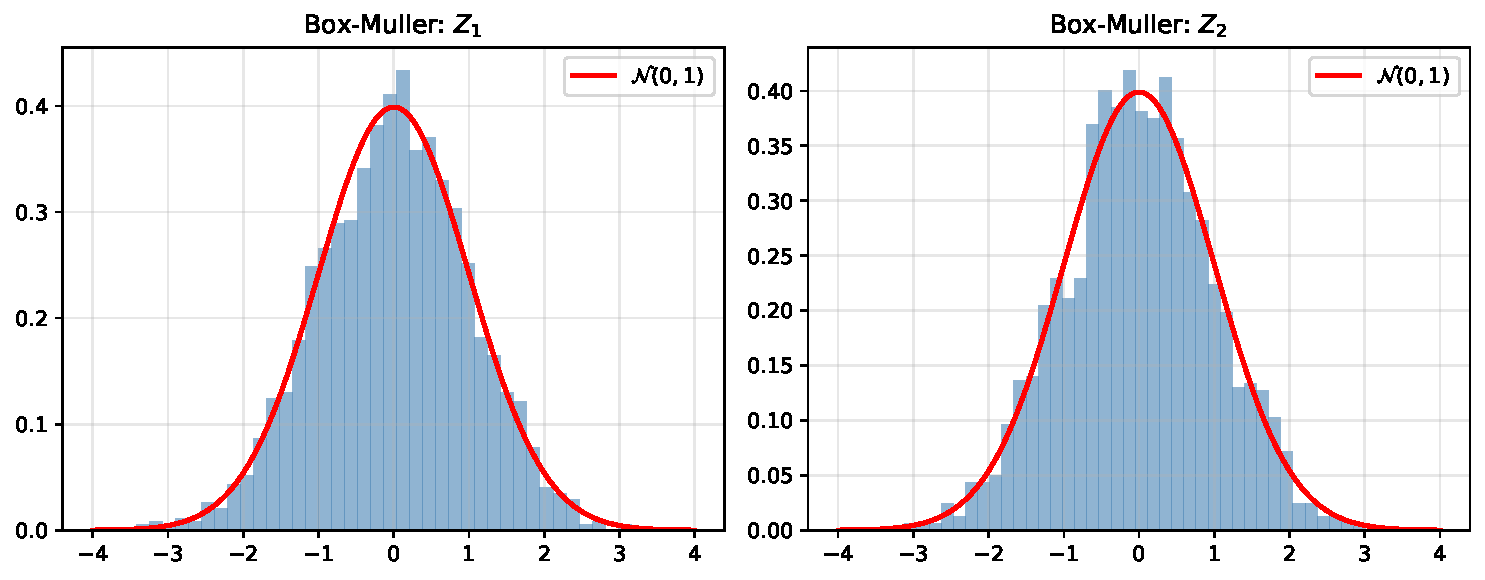
\includegraphics[width=0.62\textwidth]{fig_box_muller}
  \caption{Box-Muller output: histograms of $Z_1$ (left panel) and $Z_2$ (right
    panel) from $5\,000$ draws using Algorithm 20, overlaid with the standard
    normal density $\phi(z) = (2\pi)^{-1/2} e^{-z^2/2}$ (curve).  Both
    histograms closely match the theoretical density.}
\end{figure}

\end{frame}

\begin{frame}[allowframebreaks]{3.7.1 Marsaglia-Bray Method}

The Box-Muller method requires computing $\cos$ and $\sin$, which are slow on
older hardware (each involving many arithmetic operations via Taylor series or
table lookups).  Marsaglia and Bray (1964) proposed a variant that avoids all
trigonometric functions by generating the polar angle implicitly from uniform
random points inside the unit disc.

\textbf{Key observation.}  If $(W_1, W_2)$ is uniform on the unit disc $B_2$,
then its polar coordinates $(D', \Theta')$ satisfy $D'^2 \sim \UU[0,1)$ and
$\Theta' \sim \UU[0, 2\pi)$, and they are independent.  Moreover,
$\cos\Theta' = W_1/D'$ and $\sin\Theta' = W_2/D'$ are obtained without
any trigonometric evaluation --- we just normalize the vector $(W_1, W_2)$.

\begin{block}{Proposition 3.7.4 --- Marsaglia-Bray Transform}
  Let $V_1, V_2 \stackrel{\text{i.i.d.}}{\sim} \UU[-1,1)$ and set $X' = V_1^2 + V_2^2$.
  Conditional on $X' \le 1$ (i.e.\ the point $(V_1, V_2)$ falls inside the unit disc),
  define $Y = \sqrt{-2\log(X')/X'}$ and set:
  \[
    Z_1 = V_1 \cdot Y, \qquad Z_2 = V_2 \cdot Y.
  \]
  Then $Z_1$ and $Z_2$ are independent $\NN(0,1)$ random variables.
\end{block}

\begin{block}{Notation for Marsaglia-Bray}
  \begin{itemize}
    \item $V_1, V_2 \sim \UU[-1,1)$: uniform on $[-1, 1)$, generated as
      $V_i = 2U_i - 1$ from $U_i \sim \UU[0,1)$.
    \item $X' = V_1^2 + V_2^2$: the squared distance from the origin;
      we only proceed if $X' \le 1$ (point is inside the unit disc).
    \item $Y = \sqrt{-2\log(X')/X'}$: the Box-Muller radius $D = \sqrt{-2\log(X')}$,
      divided by $D' = \sqrt{X'}$, giving the factor $D/D'$ that converts
      Cartesian coordinates to the correctly scaled output.
  \end{itemize}
\end{block}

\begin{alertblock}{Algorithm 21 (MB): Generate $Z_1, Z_2 \sim \NN(0,1)$}
  \begin{enumerate}
    \item \textbf{Repeat:} generate $U_1, U_2$ i.i.d.\ $\UU[0,1)$;
          set $V_1 = 2U_1 - 1$, $V_2 = 2U_2 - 1$; compute $X' = V_1^2 + V_2^2$.
    \item \textbf{Until} $X' \le 1$ (the point lies inside the unit disc).
    \item Compute $Y \leftarrow \sqrt{-2\log(X')/X'}$.
    \item Compute $Z_1 \leftarrow V_1 Y$ and $Z_2 \leftarrow V_2 Y$.
    \item Return $(Z_1, Z_2)$.
  \end{enumerate}
  The acceptance probability is $\PP(V_1^2 + V_2^2 \le 1) = \pi/4 \approx 78.5\%$
  (the area of the unit disc divided by the area of the $2 \times 2$ square),
  so on average $4/\pi \approx 1.27$ pairs $(V_1, V_2)$ are generated per
  accepted pair.
\end{alertblock}

\begin{columns}
  \column{0.5\textwidth}
  \begin{figure}
    \centering
    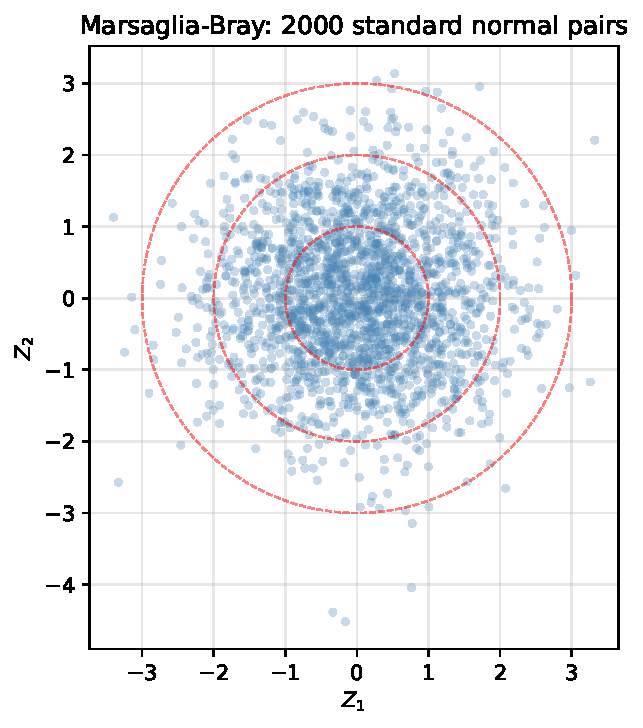
\includegraphics[width=\textwidth]{fig_marsaglia_bray}
    \caption{Scatter plot of $2\,000$ $(Z_1, Z_2)$ pairs from the Marsaglia-Bray
      method, showing the expected symmetric (isotropic) normal cloud centered
      at the origin.}
  \end{figure}
  \column{0.48\textwidth}
  \begin{alertblock}{Box-Muller vs.\ Marsaglia-Bray}
    \textbf{Box-Muller:} requires $\cos$ and $\sin$ (slow on older hardware);
    accepts every proposal (no rejections).

    \textbf{Marsaglia-Bray:} no trigonometric functions; approximately $21.5\%$
    of proposals are rejected (outside the disc).

    On modern CPUs with fast trig instructions, Box-Muller is competitive.
    On older hardware, embedded systems, or in compiled low-level code,
    Marsaglia-Bray is often faster.  Both produce exact $\NN(0,1)$ samples
    (not approximations).
  \end{alertblock}
\end{columns}

\end{frame}

\begin{frame}[allowframebreaks]{3.7.2 ITM for Normal Variables --- Numerical Inversion of $\Phi$}

To generate $Z \sim \NN(0,1)$ via the inverse transform method, we need the
quantile function $\Phi^{-1}(u)$, where $\Phi$ (Phi, uppercase) is the
standard normal c.d.f.\ $\Phi(x) = \PP(Z \le x) = \int_{-\infty}^x \frac{1}{\sqrt{2\pi}}e^{-t^2/2}\,dt$.
Unlike the exponential or Pareto, there is no closed-form expression for
$\Phi^{-1}$ and numerical methods are required.

\textbf{Newton's method.}  Given a target quantile $u$, we want to solve
$\Phi(x) = u$ for $x$.  Newton's method iterates:
\[
  x_{n+1} = x_n + (u - \Phi(x_n))\,e^{x_n^2/2 + c}, \qquad
  c = \log\!\sqrt{2\pi},
\]
since the derivative of $\Phi$ is the normal density $\phi(x_n) = e^{-x_n^2/2}/\sqrt{2\pi}$,
so $1/\phi(x_n) = e^{x_n^2/2}\sqrt{2\pi}$.  A good starting point is:
\[
  x_0 = \pm\sqrt{-1.6\log(1.0004 - (1 - 2u)^2)},
\]
and one Newton step achieves errors below $10^{-15}$.

The \textbf{Beasley-Springer-Moro} (BSM) algorithm (Algorithm 22) is a highly
optimised rational-function approximation used in practice.  For central values
$|u - 0.5| < 0.42$, it applies a rational function of $(u - 0.5)^2$.  In the
tails ($|u - 0.5| \ge 0.42$), it switches to a polynomial in $\log(-\log r)$
where $r = \min(u, 1-u)$.  This achieves absolute errors below $4 \times 10^{-9}$
across the entire range $(0,1)$ and is the basis of \texttt{scipy.stats.norm.ppf}.

\begin{alertblock}{Key Insight: When to Use ITM for Normals}
  The ITM approach via BSM or Newton is the method of choice when generating
  \emph{large batches} of normal samples in a vectorized (SIMD) setting,
  because polynomial and rational approximations are highly parallelizable
  over arrays.  Box-Muller and Marsaglia-Bray produce two samples per
  call and are better suited for sequential loops.  NumPy's
  \texttt{rng.standard\_normal()} uses a variant of this numerical inversion.
\end{alertblock}

\end{frame}

\begin{frame}[allowframebreaks]{3.7.3 Multivariate Normal $\NN(\boldsymbol{\mu}, \boldsymbol{\Sigma})$}

A random vector $\mathbf{X} \in \RR^d$ has the multivariate normal distribution
$\NN(\boldsymbol{\mu}, \boldsymbol{\Sigma})$ if every linear combination
$\mathbf{a}^T \mathbf{X} = a_1 X_1 + \cdots + a_d X_d$ is univariate normal.

\begin{block}{Notation: Multivariate Normal}
  \begin{itemize}
    \item $\boldsymbol{\mu}$ (mu): the $d$-dimensional \emph{mean vector},
      $\boldsymbol{\mu} = (\mu_1, \ldots, \mu_d)^T$, where $\mu_i = \EE[X_i]$.
    \item $\boldsymbol{\Sigma}$ (Sigma): the $d \times d$ \emph{covariance matrix}.
      Its $(i,j)$ entry is $\Sigma_{ij} = \mathrm{Cov}(X_i, X_j) = \EE[(X_i - \mu_i)(X_j - \mu_j)]$.
      The diagonal entries $\Sigma_{ii} = \mathrm{Var}(X_i)$ are the individual variances.
    \item $\boldsymbol{\Sigma}$ must be symmetric and positive semidefinite
      (all eigenvalues $\ge 0$).
  \end{itemize}
\end{block}

The key structural fact is that any $\NN(\boldsymbol{\mu}, \boldsymbol{\Sigma})$
vector can be obtained from a vector of independent standard normals by a linear
transformation.  This is the basis of the simulation algorithm.

\begin{block}{Proposition 3.7.8 --- Cholesky Method for Multivariate Normal}
  Every symmetric positive semidefinite matrix $\boldsymbol{\Sigma}$ can be
  factored as $\boldsymbol{\Sigma} = \mathbf{A}\mathbf{A}^T$, where $\mathbf{A}$
  is a lower-triangular matrix (the \emph{Cholesky factor}).
  If $\mathbf{Z} = (Z_1, \ldots, Z_d)^T$ is a vector with i.i.d.\ $Z_i \sim \NN(0,1)$,
  then:
  \[
    \mathbf{X} = \mathbf{A}\mathbf{Z} + \boldsymbol{\mu}
    \;\sim\; \NN(\boldsymbol{\mu},\boldsymbol{\Sigma}).
  \]
\end{block}

\textbf{Proof.}
$\EE[\mathbf{X}] = \mathbf{A}\EE[\mathbf{Z}] + \boldsymbol{\mu} = \boldsymbol{\mu}$
(since $\EE[\mathbf{Z}] = \mathbf{0}$).
$\mathrm{Cov}(\mathbf{X}) = \mathbf{A}\,\mathrm{Cov}(\mathbf{Z})\,\mathbf{A}^T
= \mathbf{A}\,\mathbf{I}\,\mathbf{A}^T = \mathbf{A}\mathbf{A}^T = \boldsymbol{\Sigma}$,
where $\mathbf{I}$ is the identity matrix and $\mathrm{Cov}(\mathbf{Z}) = \mathbf{I}$
because the components of $\mathbf{Z}$ are independent with unit variance.

\begin{alertblock}{How to Read $\mathbf{X} = \mathbf{A}\mathbf{Z} + \boldsymbol{\mu}$}
  The Cholesky factor $\mathbf{A}$ is a ``stretching and rotating'' matrix that
  transforms the spherically symmetric standard normal cloud $\mathbf{Z}$ into
  an ellipsoidal cloud aligned with the correlations specified by $\boldsymbol{\Sigma}$.
  Adding $\boldsymbol{\mu}$ shifts the centre of the cloud to the desired mean.
\end{alertblock}

\framebreak

\textbf{Bivariate case ($d = 2$).}
With $\boldsymbol{\Sigma} = \begin{pmatrix}\sigma_1^2 & \rho\sigma_1\sigma_2 \\ \rho\sigma_1\sigma_2 & \sigma_2^2\end{pmatrix}$,
where $\rho$ (rho) is the correlation coefficient ($-1 < \rho < 1$), $\sigma_1$ (sigma one)
and $\sigma_2$ (sigma two) are the standard deviations of $X_1$ and $X_2$ respectively.
Using the Cholesky factor, the simulation formula is:
\[
  X_1 = \sigma_1\!\left(\sqrt{1-|\rho|}\,Z_1 + \sqrt{|\rho|}\,Z_3\right), \quad
  X_2 = \sigma_2\!\left(\sqrt{1-|\rho|}\,Z_2 + \mathrm{sign}(\rho)\sqrt{|\rho|}\,Z_3\right),
\]
where $Z_1, Z_2, Z_3$ are three independent $\NN(0,1)$ random variables.
The shared component $Z_3$ introduces the correlation between $X_1$ and $X_2$.

\begin{figure}
  \centering
  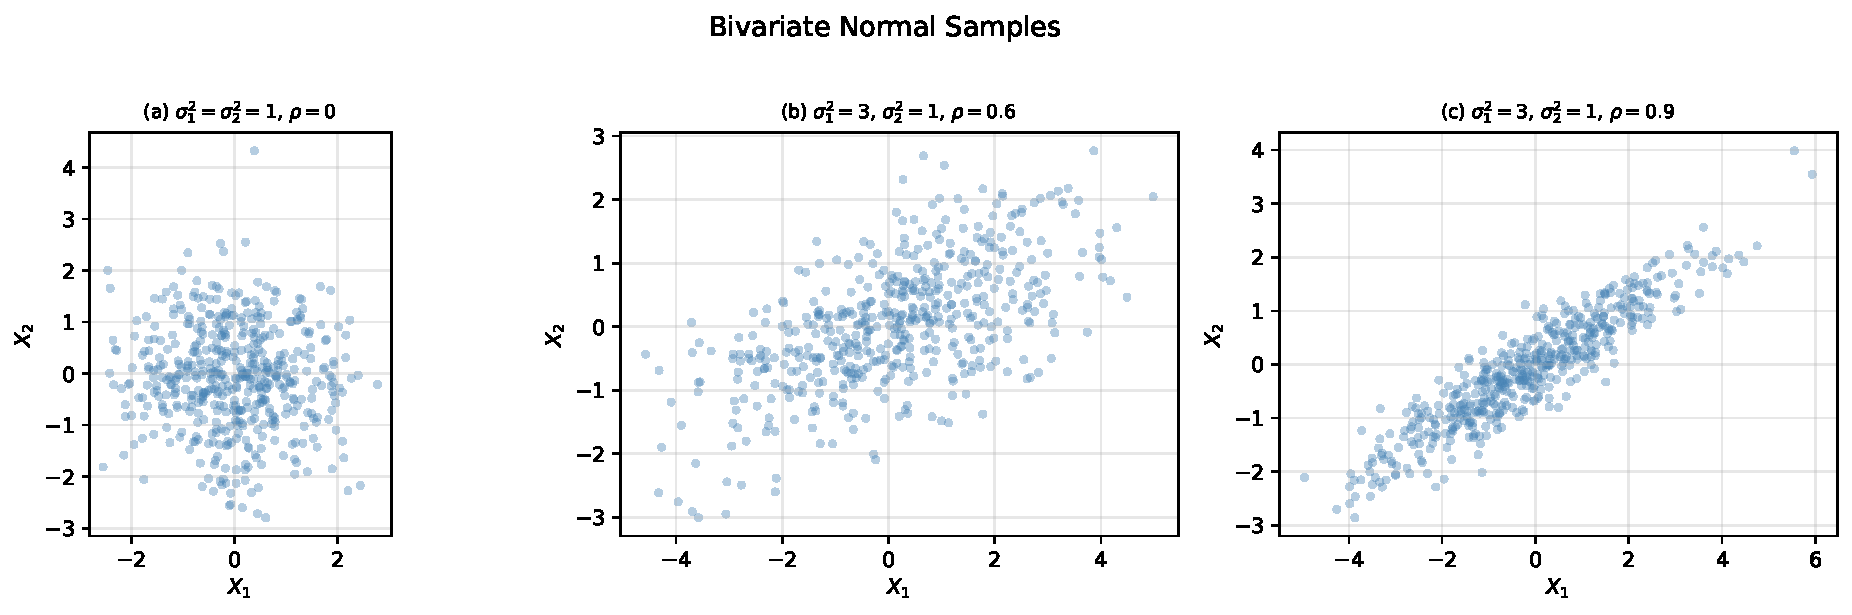
\includegraphics[width=0.82\textwidth]{fig_bivariate_normal}
  \caption{$500$ samples from $\NN(\mathbf{0}, \boldsymbol{\Sigma})$ for three
    covariance settings.  (a) $\sigma_1^2 = \sigma_2^2 = 1$, $\rho = 0$: the
    cloud is a symmetric circle (no correlation).
    (b) $\sigma_1^2 = 3$, $\sigma_2^2 = 1$, $\rho = 0.6$: the cloud is an
    elongated ellipse tilted toward the upper right.
    (c) $\rho = 0.9$: strong positive correlation, the cloud is very elongated.}
\end{figure}

\end{frame}

\begin{frame}[fragile]{3.7 Python: Multivariate Normal via Cholesky}
\begin{lstlisting}[style=python, caption={Multivariate normal sampling via Cholesky decomposition (Proposition 3.7.8)}]
import numpy as np
rng = np.random.default_rng(42)

def sample_multivariate_normal(mu, Sigma, n, rng):
    """
    Generate n samples from N(mu, Sigma) using the Cholesky method.
    Proposition 3.7.8: X = A*Z + mu, where Sigma = A @ A.T.
    A is the lower-triangular Cholesky factor.
    """
    d = len(mu)
    A = np.linalg.cholesky(Sigma)    # A is lower-triangular
    Z = rng.standard_normal((d, n))  # d x n matrix of i.i.d. N(0,1)
    return (A @ Z).T + mu            # shape: (n, d)

# 2D example: mean [1,-2], covariance with rho=0.849
mu    = np.array([1.0, -2.0])
Sigma = np.array([[2.0, 1.2],
                  [1.2, 1.0]])  # rho = 1.2/sqrt(2*1) = 0.849

samples = sample_multivariate_normal(mu, Sigma, 2000, rng)
print("Empirical mean:", samples.mean(axis=0).round(3))
# Expected: approx [1.0, -2.0]
print("Empirical covariance:\n", np.cov(samples.T).round(3))
# Expected: approx [[2.0, 1.2], [1.2, 1.0]]
\end{lstlisting}
\end{frame}

% ============================================================
\section{3.8 Uniform Distribution on Balls, Spheres, Ellipsoids}
% ============================================================

\begin{frame}[allowframebreaks]{3.8 Geometry: Balls, Spheres, and Their Volumes}

This section develops algorithms to sample uniformly from geometric objects ---
the $d$-ball, the $(d-1)$-sphere, and ellipsoids --- without relying on the
rejection-from-bounding-box method, which is exponentially inefficient in high
dimensions (as we saw in Section 3.4).

\begin{block}{Key Geometric Objects and Their Volumes}
  \begin{align*}
    B_d &= \{\mathbf{x} \in \RR^d : x_1^2 + \cdots + x_d^2 \le 1\}
    &&\text{(the $d$-dimensional unit ball)}, \\
    S_{d-1} &= \{\mathbf{x} \in \RR^d : x_1^2 + \cdots + x_d^2 = 1\}
    &&\text{(the $(d-1)$-dimensional unit sphere)}.
  \end{align*}
  Their volumes (measures) are:
  \[
    \Vol(B_d) = \frac{\pi^{d/2}}{\Gamma(d/2+1)}, \qquad
    \mathrm{Area}(S_{d-1}) = \frac{2\pi^{d/2}}{\Gamma(d/2)}.
  \]
  Here $\Gamma$ (Gamma) is the gamma function, satisfying $\Gamma(n) = (n-1)!$
  for positive integers $n$ and $\Gamma(1/2) = \sqrt{\pi}$.
\end{block}

\begin{block}{Notation}
  \begin{itemize}
    \item $B_d$ (ball): all points \emph{at or inside} the unit sphere.
    \item $S_{d-1}$ (sphere): only points \emph{on} the surface of the unit sphere.
      The sphere $S_{d-1}$ is $(d-1)$-dimensional (a surface), embedded in
      $d$-dimensional space $\RR^d$.  For example, $S_2$ is the familiar
      2D surface of a ball in 3D space.
    \item $\pi^{d/2}$: pi to the power $d/2$; grows, but $\Gamma(d/2+1)$ grows
      faster, so $\Vol(B_d) \to 0$ as $d \to \infty$.
  \end{itemize}
\end{block}

\textbf{Surface area element (Lemma 3.8.8).}
For a surface parametrised as $\mathbf{x}(\mathbf{t})$ with Jacobian matrix
$\mathbf{J}(\mathbf{t}) = (\partial x_j/\partial t_i)_{i,j}$,
the surface area element is $dA = \sqrt{|\det(\mathbf{J}\mathbf{J}^T)|}\,d\mathbf{t}$.
This generalises the standard change-of-variables Jacobian to
lower-dimensional surfaces embedded in $\RR^d$.

\end{frame}

\begin{frame}[allowframebreaks]{3.8.1 Sampling Uniformly on $S_2$ and in $B_3$}

For $d = 3$, the sphere $S_2$ (the surface of the unit ball in 3D) is parametrised
by spherical coordinates: $(\theta, \phi) \in [0,2\pi) \times [0,\pi)$, with
\[
  x = \cos\theta\sin\phi, \quad y = \sin\theta\sin\phi, \quad z = \cos\phi.
\]
Here $\theta$ (theta) is the azimuthal angle (longitude) and $\phi$ (phi) is the
polar angle (colatitude, measured from the north pole).  The surface area element is
$dA = \sin\phi\,d\phi\,d\theta$.

\textbf{Important:} sampling $\phi$ uniformly on $[0, \pi)$ would \emph{not}
give a uniform distribution on the sphere!  Points near the poles ($\phi \approx 0$
or $\phi \approx \pi$) are closer together (the area element $\sin\phi$ is small
there), so they need to be sampled less frequently.  The correct density for $\phi$
is $f(\phi) = \frac{1}{2}\sin\phi$, which has c.d.f.\ $F_\Phi(\phi) = (1-\cos\phi)/2$.
Inverting: $\phi = \arccos(1 - 2V)$ for $V \sim \UU[0,1)$.
The azimuthal angle $\theta = 2\pi W$ for independent $W \sim \UU[0,1)$.

\begin{block}{Proposition 3.8.6 --- The Normal Trick for $\UU(S_2)$}
  If $Z_1, Z_2, Z_3 \stackrel{\text{i.i.d.}}{\sim} \NN(0,1)$, then the normalised
  vector
  \[
    \mathbf{X} = \frac{(Z_1, Z_2, Z_3)}{\|(Z_1,Z_2,Z_3)\|}
    = \left(\frac{Z_1}{\|\mathbf{Z}\|},\, \frac{Z_2}{\|\mathbf{Z}\|},\,
    \frac{Z_3}{\|\mathbf{Z}\|}\right)
    \;\sim\; \UU(S_2).
  \]
\end{block}

\textbf{Why this works.}  The density of $\mathbf{Z} = (Z_1, Z_2, Z_3)$ is
$f(\mathbf{z}) \propto e^{-\|\mathbf{z}\|^2/2}$, which depends only on the
radius $\|\mathbf{z}\|$ and not on the direction $\mathbf{z}/\|\mathbf{z}\|$.
This \emph{spherical symmetry} means that the direction is uniformly distributed
on $S_2$, independent of the radius.  Normalising removes the radius, leaving
a $\UU(S_2)$ sample.

\framebreak

The Normal trick generalises immediately to any dimension $d$.

\begin{block}{General Algorithms: $\UU(S_{d-1})$ and $\UU(B_d)$}
  \textbf{Sampling uniformly on the $(d-1)$-sphere $S_{d-1}$:}
  \begin{enumerate}
    \item Generate $\mathbf{Z} = (Z_1, \ldots, Z_d)^T$ with i.i.d.\ $Z_i \sim \NN(0,1)$.
    \item Return $\mathbf{X} = \mathbf{Z}/\|\mathbf{Z}\|$.
  \end{enumerate}

  \textbf{Sampling uniformly in the $d$-ball $B_d$ (Proposition 3.8.13):}
  \begin{enumerate}
    \item Sample $\mathbf{S} \sim \UU(S_{d-1})$ using the steps above.
    \item Independently sample $U \sim \UU[0,1)$.
    \item Return $\mathbf{X} = U^{1/d}\,\mathbf{S}$.
  \end{enumerate}
  The scaling $U^{1/d}$ (U to the power one over d) ensures uniformity inside
  the ball.  The c.d.f.\ of the radius $R = \|\mathbf{X}\|$ must be $F_R(r) = r^d$
  for $r \in [0,1]$ (since volume scales as $r^d$), and ITM gives $R = U^{1/d}$.
\end{block}

\begin{alertblock}{How to Read the Scaling $U^{1/d}$}
  In one dimension ($d=1$), $U^{1/1} = U$ --- a uniform radius, which is correct
  for a line segment.  In two dimensions ($d=2$), $U^{1/2} = \sqrt{U}$ --- most
  of the area of a disc is near the boundary, so the radius must be biased toward
  1.  In high dimensions, $U^{1/d}$ concentrates near 1 for large $d$, reflecting
  the fact that almost all of the volume of a high-dimensional ball is near the
  surface (the ``hollow ball'' phenomenon).
\end{alertblock}

\begin{figure}
  \centering
  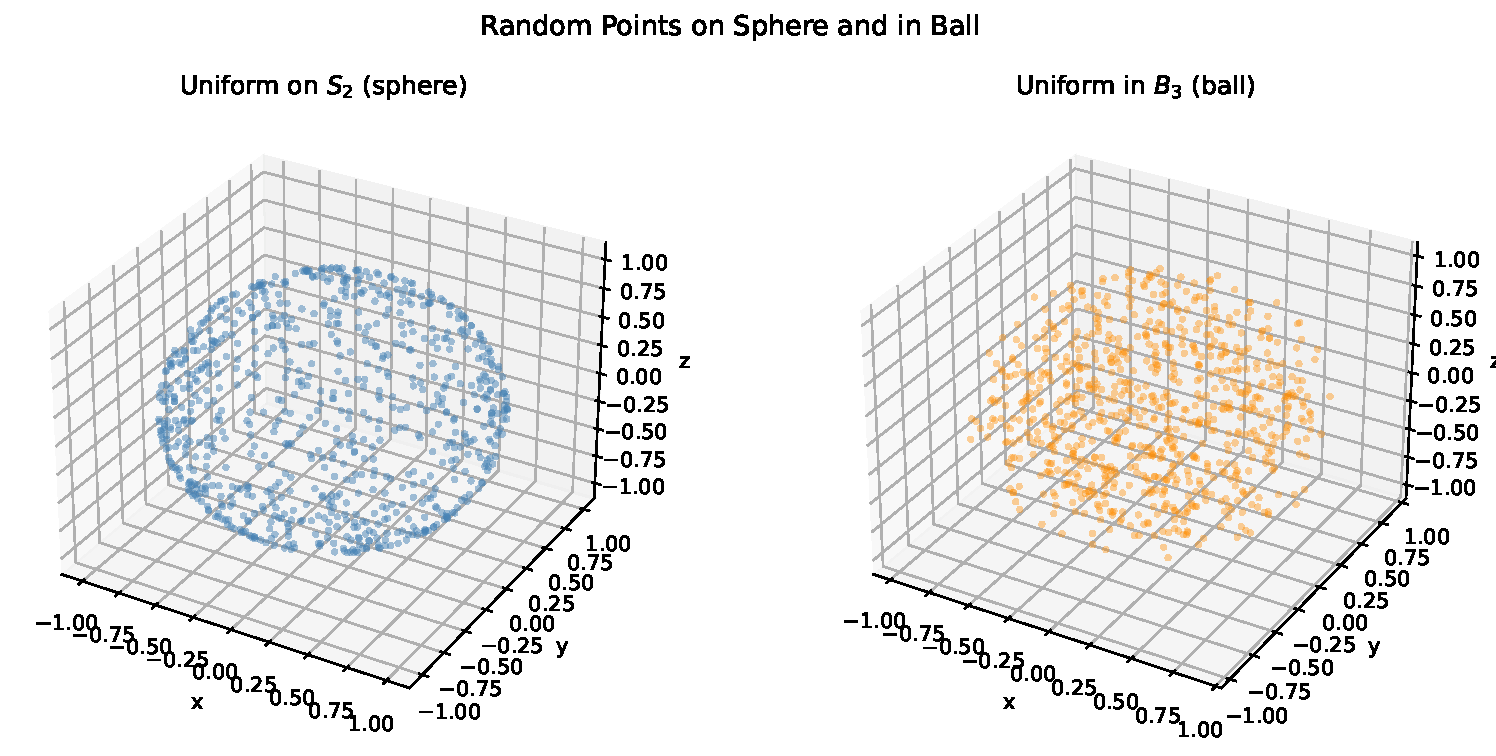
\includegraphics[width=0.60\textwidth]{fig_ball_sphere}
  \caption{Left: $1\,000$ uniform random points on $S_2$ (the unit sphere surface
    in 3D) generated by the Normal trick.  Right: $1\,000$ uniform random points
    inside $B_3$ (the unit ball in 3D) generated by the Normal trick followed by
    scaling by $U^{1/3}$.}
\end{figure}

\end{frame}

\begin{frame}[fragile]{3.8 Python: Sphere and Ball Sampling}
\begin{lstlisting}[style=python, caption={Uniform sampling on the (d-1)-sphere and d-ball via the Normal trick}]
import numpy as np
rng = np.random.default_rng(42)

def sample_sphere(d, n, rng):
    """
    Uniform on the (d-1)-sphere S_{d-1} in R^d.
    Method: normalise d independent N(0,1) variables.
    The spherical symmetry of N(0,I) ensures uniform direction.
    """
    Z = rng.standard_normal((n, d))
    norms = np.linalg.norm(Z, axis=1, keepdims=True)
    return Z / norms    # each row has norm exactly 1

def sample_ball(d, n, rng):
    """
    Uniform inside the d-ball B_d in R^d.
    Method: X = U^(1/d) * (point on sphere).
    Scaling U^(1/d) gives CDF F_R(r) = r^d on [0,1],
    matching the volume growth r^d of a d-ball.
    """
    S = sample_sphere(d, n, rng)           # uniform direction
    U = rng.uniform(0, 1, n)[:, None]     # uniform radius before scaling
    return S * (U ** (1.0 / d))           # scale to get uniform in ball

# Verification
pts_sphere = sample_sphere(3, 5000, rng)
pts_ball   = sample_ball(3, 5000, rng)
norms_sph = np.linalg.norm(pts_sphere, axis=1)
norms_bal = np.linalg.norm(pts_ball,   axis=1)
print(f"Sphere norms (should all be 1.000): mean={norms_sph.mean():.4f}")
print(f"Ball mean radius (theory: d/(d+1) = 0.750): {norms_bal.mean():.4f}")
\end{lstlisting}
\end{frame}

\begin{frame}[allowframebreaks]{3.8.3 Sampling Uniformly Within an Ellipsoid}

An ellipsoid $\mathcal{E}_d = \{\mathbf{x} \in \RR^d : \mathbf{x}^T \mathbf{A}^{-1} \mathbf{x} \le 1\}$
is a linearly stretched version of the unit ball, where $\mathbf{A}$ is a
symmetric positive-definite matrix.  The volume of $\mathcal{E}_d$ is
$\Vol(B_d) \cdot \sqrt{\det \mathbf{A}}$.

\textbf{Notation:}  $\mathbf{x}^T \mathbf{A}^{-1} \mathbf{x}$ (x-transpose times
$A$-inverse times $x$) is a \emph{quadratic form}; it measures the ``distance''
of $\mathbf{x}$ from the origin in the metric defined by $\mathbf{A}^{-1}$.
The condition $\mathbf{x}^T \mathbf{A}^{-1} \mathbf{x} \le 1$ defines the
interior of the ellipsoid.

\textbf{Key idea.}  Factorise $\mathbf{A} = \mathbf{L}\mathbf{L}^T$ (Cholesky
decomposition).  The map $\mathbf{x} \mapsto \mathbf{L}^{-1}\mathbf{x}$ transforms
$\mathcal{E}_d$ bijectively (one-to-one and onto) into the unit ball $B_d$.
Therefore: sample $\mathbf{X} \sim \UU(B_d)$ and return $\mathbf{Y} = \mathbf{L}\mathbf{X}$,
which is then uniform in $\mathcal{E}_d$.

\begin{block}{Algorithm 23 --- $\UU(\mathcal{E}_d)$: Uniform in an Ellipsoid}
  \begin{enumerate}
    \item Factorise $\mathbf{A} = \mathbf{L}\mathbf{L}^T$ (Cholesky decomposition,
          or spectral $\mathbf{A} = \mathbf{P}\,\mathrm{diag}(\mathbf{a}^2)\,\mathbf{P}^T$).
    \item Generate $\mathbf{X} \sim \UU(B_d)$ using the Normal trick.
    \item Return $\mathbf{Y} = \mathbf{L}\mathbf{X}$.
  \end{enumerate}
\end{block}

\begin{exampleblock}{Worked 2D Example}
  For the ellipse $(x/3)^2 + (y/1)^2 \le 1$ with semi-axes $a = 3$ and $b = 1$:
  the matrix is $\mathbf{A} = \mathrm{diag}(9, 1)$ and
  $\mathbf{L} = \mathrm{diag}(3, 1)$.
  Sample $(X_1, X_2) \sim \UU(B_2)$, then return $(Y_1, Y_2) = (3X_1, X_2)$.
  This stretches the circular sample by a factor of 3 in the $x$-direction.
\end{exampleblock}

\begin{figure}
  \centering
  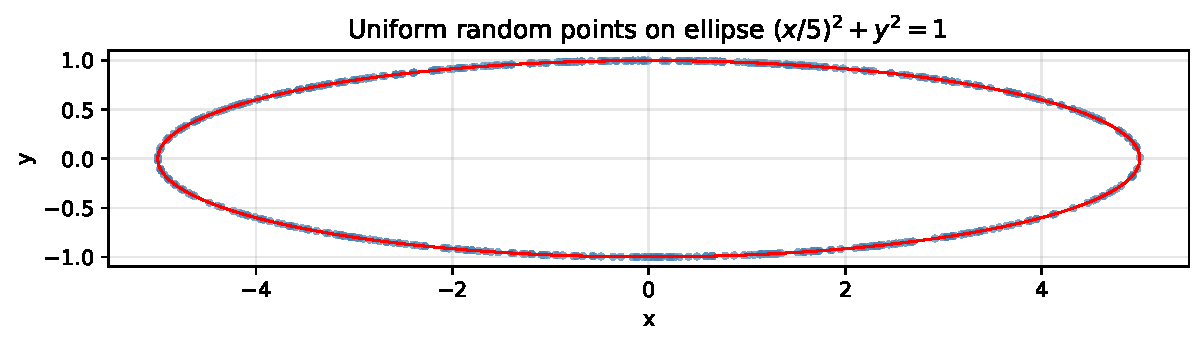
\includegraphics[width=0.48\textwidth]{fig_ellipse_uniform}
  \caption{$1\,000$ uniform random points within the ellipse $(x/3)^2 + y^2 \le 1$
    generated by Algorithm 23: sample uniformly in the unit disc, then apply the
    linear map $(X_1, X_2) \mapsto (3X_1, X_2)$.}
\end{figure}

\end{frame}

\begin{frame}[allowframebreaks]{3.8.4--3.8.5 Sampling on Ellipsoid Surfaces and Average Shadow}

\textbf{Sampling on the surface of a 3D ellipsoid.}
Consider the ellipsoid surface
$\frac{x^2}{a^2} + \frac{y^2}{b^2} + \frac{z^2}{c^2} = 1$,
parametrised by $(\theta, \phi) \in [0,2\pi) \times [0,\pi)$:
\[
  \mathbf{x}(\theta,\phi) = (a\cos\theta\sin\phi,\; b\sin\theta\sin\phi,\; c\cos\phi).
\]
The area element $dA = \sqrt{g(\phi,\theta)}\,d\phi\,d\theta$ where
$\sqrt{g} = \sin\phi\sqrt{c^2(a^2\sin^2\phi\sin^2\theta + b^2\sin^2\phi\cos^2\theta) + a^2 b^2 \cos^2\phi}$
does \emph{not} separate into a product of a function of $\theta$ and a function of
$\phi$ when $a, b, c$ are all different.  Therefore, $\theta$ and $\phi$ cannot
be sampled independently.  Algorithm 24 uses a numerical approach: subdivide the
parameter rectangle into a grid, approximate each cell's area using a cross-product
of tangent vectors, then sample a cell proportional to its area and place a uniform
point within it.

\textbf{Average shadow of a 3D body (Section 3.8.5).}
The \emph{shadow} (projection) of a planar face $F$ cast by parallel light arriving
from direction $\mathbf{n}$ has area equal to $|\cos\angle(\mathbf{n}, \hat{\mathbf{n}}_F)| \cdot \mathrm{Area}(F)$,
where $\hat{\mathbf{n}}_F$ is the outward normal of the face.

\begin{block}{Expected Shadow Formula}
  For a single flat face $F$ with the light direction drawn uniformly from $S_2$:
  \[
    \EE[\mathrm{Area}(\mathrm{shadow}(F))] = \frac{\mathrm{Area}(F)}{2}.
  \]
  For a convex polyhedron with faces $F_1, \ldots, F_m$ and light direction drawn
  uniformly from all directions:
  \[
    \EE[\mathrm{Area}(\mathrm{shadow})] = \frac{\mathrm{surface\;area}}{4}.
  \]
  For a unit cube (surface area $= 6$): $\EE[\mathrm{shadow}] = 6/4 = 3/2$.
\end{block}

\textbf{Derivation.}  For a single face, we need $\EE[|\cos\phi|\sin\phi]$ where
the polar angle $\phi$ (phi) has density $f(\phi) = \frac{1}{2}\sin\phi$ on
$[0,\pi)$ (uniform on $S_2$).  This integral evaluates to $1/2$, giving the
factor of $1/2$ for each face.  Summing over all faces and noting that each face
points ``outward'' for half of all light directions (the other half hit the opposite
side and cast no shadow) gives the overall factor of $1/4$.

\end{frame}

% ============================================================
\section{3.9 Bivariate Vectors: Conditional ITM and Copulas}
% ============================================================

\begin{frame}[allowframebreaks]{3.9.1 Conditional Inverse Transform Method}

When we need to simulate a \emph{bivariate} random vector $(X, Y)$ with a
specified joint density $f(x, y)$, one natural approach is the
\emph{conditional ITM}: first simulate the marginal distribution of $X$,
then simulate $Y$ from the conditional distribution of $Y$ given $X$.
This leverages the fundamental identity
$f(x, y) = f_X(x) \cdot f_{Y|X=x}(y)$ to decompose the joint sampling
into two simpler one-dimensional problems.

\begin{block}{Algorithm --- Conditional ITM for $(X, Y)$}
  \begin{enumerate}
    \item Compute the marginal density $f_X(x) = \int_{-\infty}^{+\infty} f(x,y)\,dy$
          and its c.d.f.\ $F_X$.
    \item Generate $X = F_X^{\leftarrow}(U_1)$ for independent $U_1 \sim \UU[0,1)$.
    \item Given $X = \mathsf{x}$, compute the conditional c.d.f.\
          $F_{Y|X=\mathsf{x}}(y) = \int_{-\infty}^y \frac{f(\mathsf{x},t)}{f_X(\mathsf{x})}\,dt$.
    \item Generate $Y = F_{Y|X=\mathsf{x}}^{\leftarrow}(U_2)$ for independent $U_2 \sim \UU[0,1)$.
    \item Return $(X, Y)$.
  \end{enumerate}
\end{block}

\begin{exampleblock}{Example 3.9.1 --- Worked Derivation}
  Let $f(x, y) = x\,e^{-x(y+1)}$ for $x, y \ge 0$.

  \textbf{Step 1: find the marginal $f_X$.}
  \[
    f_X(x) = \int_0^\infty x\,e^{-x(y+1)}\,dy
    = x\,e^{-x} \int_0^\infty e^{-xy}\,dy
    = x\,e^{-x} \cdot \frac{1}{x} = e^{-x}.
  \]
  So $X \sim \mathrm{Exp}(1)$.  Simulation: $X = -\log U_1$.

  \textbf{Step 2: find the conditional $f_{Y|X=\mathsf{x}}$.}
  \[
    f_{Y|X=\mathsf{x}}(y)
    = \frac{f(\mathsf{x}, y)}{f_X(\mathsf{x})}
    = \frac{\mathsf{x}\,e^{-\mathsf{x}(y+1)}}{e^{-\mathsf{x}}}
    = \mathsf{x}\,e^{-\mathsf{x}y}.
  \]
  This is the density of $\mathrm{Exp}(\mathsf{x})$.  Simulation: $Y = -\log(U_2)/\mathsf{x}$.
\end{exampleblock}

\begin{figure}
  \centering
  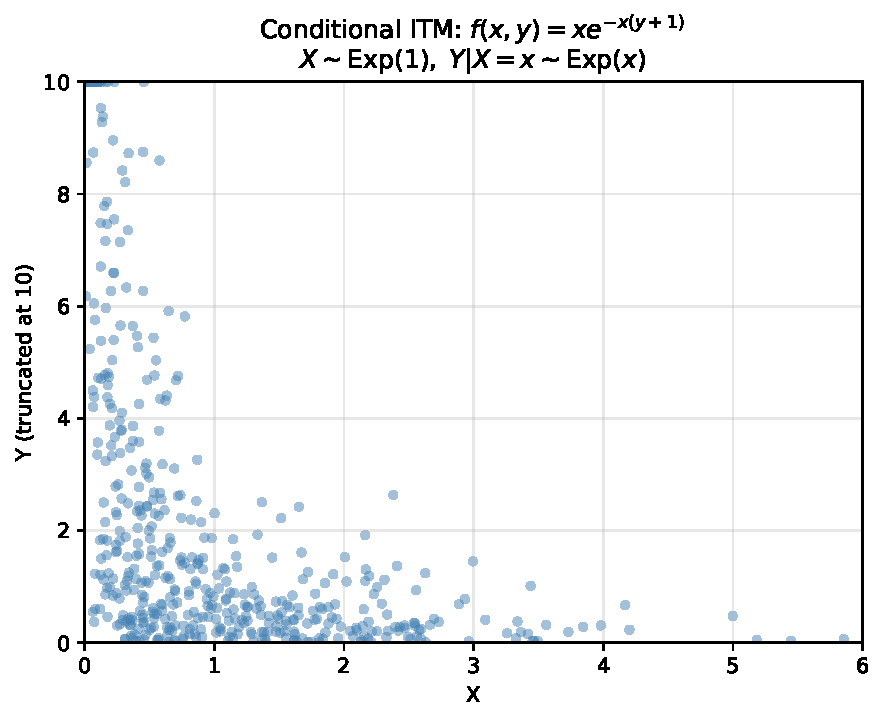
\includegraphics[width=0.42\textwidth]{fig_conditional_itm}
  \caption{$100$ samples from $f(x,y) = x\,e^{-x(y+1)}$ via the conditional ITM.
    Large values of $X$ lead to $\mathrm{Exp}(X)$ distributions for $Y$ that
    concentrate near 0, explaining the positive correlation visible in the scatter plot.}
\end{figure}

\end{frame}

\begin{frame}[allowframebreaks]{3.9.2 Bivariate Copulas and Sklar's Theorem}

Specifying a joint distribution via its density intertwines the marginal
distributions (how each variable individually behaves) and the dependence
structure (how the variables co-vary).  \emph{Copulas} provide a language for
separating these two concerns: a copula encodes only the dependence structure,
and the marginal distributions are specified separately.

\begin{block}{Definition --- Bivariate Copula}
  A \textbf{copula} is a bivariate c.d.f.\ $C: [0,1]^2 \to [0,1]$ whose
  marginal distributions are both $\UU[0,1)$.  Formally, $C$ satisfies:
  \begin{enumerate}[(a)]
    \item Boundary conditions: $C(u, 0) = C(0, v) = 0$ and $C(u, 1) = u$, $C(1, v) = v$.
    \item 2-increasing: for $u_1 \le u_2$, $v_1 \le v_2$:
          $C(u_2,v_2) - C(u_1,v_2) - C(u_2,v_1) + C(u_1,v_1) \ge 0$.
          (This ensures $C$ is a valid c.d.f., assigning non-negative probability
          to every rectangle.)
  \end{enumerate}
\end{block}

\begin{block}{Theorem 3.9.2 --- Sklar's Theorem}
  For any joint c.d.f.\ $F_{X,Y}(t_1, t_2)$ with marginals $F_X$ and $F_Y$,
  there exists a copula $C$ such that:
  \[
    F_{X,Y}(t_1, t_2) = C(F_X(t_1),\; F_Y(t_2)).
  \]
  If $F_X$ and $F_Y$ are continuous, $C$ is \emph{unique}.
  The joint density factors as:
  \[
    f_{X,Y}(t_1, t_2) = f_X(t_1)\cdot f_Y(t_2)\cdot c(F_X(t_1),\; F_Y(t_2)),
  \]
  where $c(u_1, u_2) = \partial^2 C(u_1, u_2)/\partial u_1\,\partial u_2$
  is the \textbf{copula density}.
\end{block}

\begin{alertblock}{How to Read Sklar's Theorem}
  Sklar's theorem says any joint distribution can be built in two steps:
  (1) choose the marginal distributions $F_X$ and $F_Y$ independently,
  (2) choose a copula $C$ to specify the dependence structure.
  The result is always a valid joint distribution.  Crucially, you can change
  the copula without changing the marginals, or change the marginals without
  changing the dependence structure.
\end{alertblock}

\framebreak

\begin{block}{Fr\'{e}chet-Hoeffding Bounds (Theorem 3.9.6)}
  For any bivariate copula $C(u_1, u_2)$:
  \[
    \max(u_1 + u_2 - 1,\; 0) \;\le\; C(u_1, u_2) \;\le\; \min(u_1, u_2).
  \]
  The three extreme copulas are:
  \begin{itemize}
    \item \textbf{Upper bound (perfect positive dependence):}
          $C_U(u_1, u_2) = \min(u_1, u_2)$.
          Simulation: set $V_1 = V_2 = U$ for a single $U \sim \UU[0,1)$.
          The two marginals move in lockstep (perfectly correlated).
    \item \textbf{Lower bound (perfect negative dependence):}
          $C_L(u_1, u_2) = \max(0, u_1 + u_2 - 1)$.
          Simulation: set $V_1 = U$, $V_2 = 1 - U$.
          When one is large, the other is small.
    \item \textbf{Independence:} $C_I(u_1, u_2) = u_1 u_2$.
          Simulation: set $V_1, V_2$ independent.
  \end{itemize}
\end{block}

\begin{figure}
  \centering
  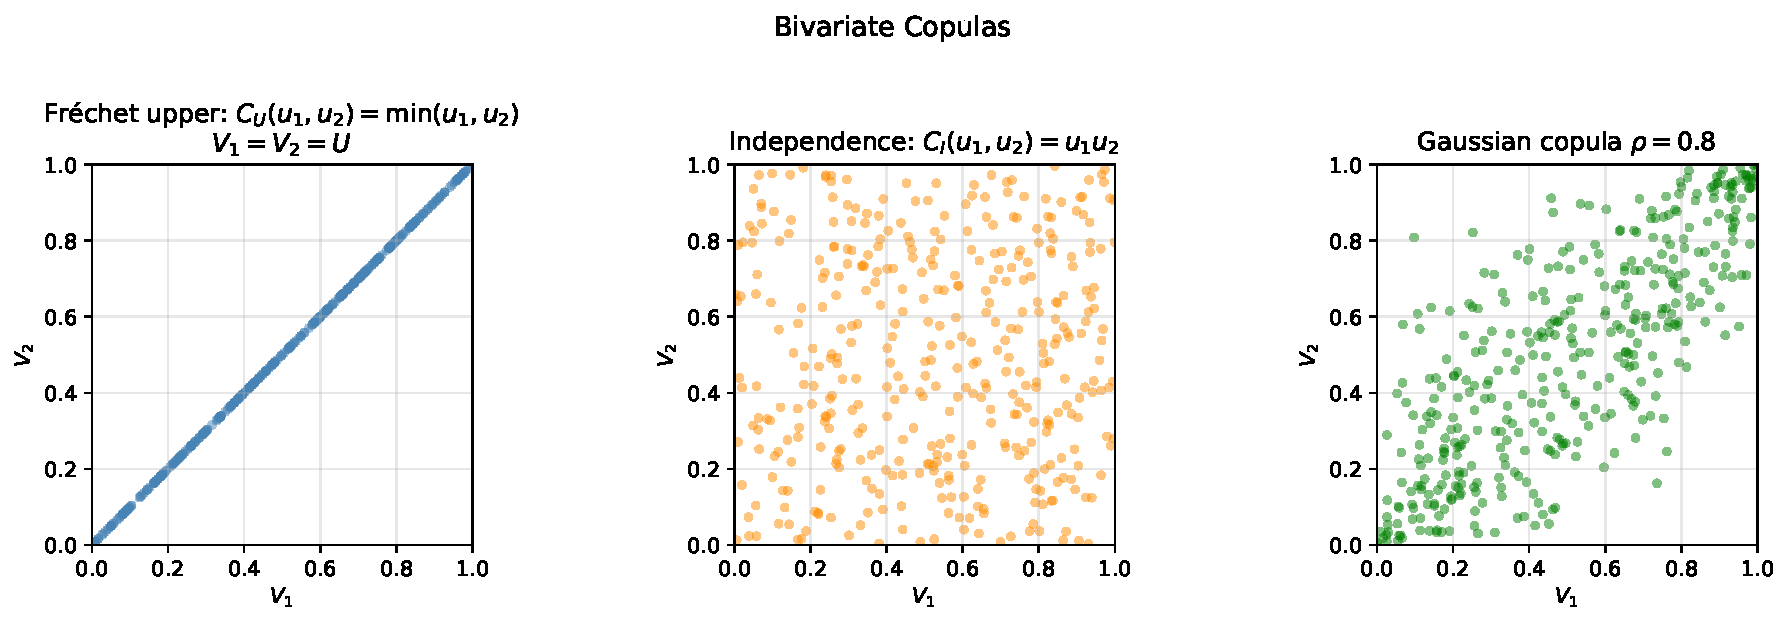
\includegraphics[width=0.72\textwidth]{fig_copulas}
  \caption{$1\,000$ samples $(V_1, V_2)$ from three copulas.
    Left: the Fr\'{e}chet upper copula $C_U$ (all points on the diagonal
    $V_1 = V_2$, perfect positive dependence).
    Centre: the independence copula $C_I$ (uniform scatter).
    Right: the Gaussian copula with $\rho = 0.8$ (elliptical cloud,
    positive dependence but not perfect).}
\end{figure}

\end{frame}

\begin{frame}[allowframebreaks]{3.9.3 Classical Copulas and Their Simulation}

\begin{block}{Gaussian (Normal) Copula}
  Let $\Phi_\rho$ (Phi sub rho) be the bivariate normal c.d.f.\ with standard
  marginals and correlation $\rho$ (rho) $\in (-1, 1)$.  The Gaussian copula is:
  \[
    C_\rho(u_1, u_2) = \Phi_\rho(\Phi^{-1}(u_1),\; \Phi^{-1}(u_2)).
  \]
  Here $\Phi^{-1}$ (capital Phi inverse) is the standard normal quantile function.

  \textbf{Simulation of $(V_1, V_2) \sim C_\rho$:}
  \begin{enumerate}
    \item Generate $(X, Y) \sim \NN(\mathbf{0}, \boldsymbol{\Sigma})$ with
          $\boldsymbol{\Sigma} = \bigl(\begin{smallmatrix}1&\rho\\\rho&1\end{smallmatrix}\bigr)$
          using the Cholesky method.
    \item Transform to uniform marginals: $(V_1, V_2) = (\Phi(X), \Phi(Y))$.
  \end{enumerate}
\end{block}

\begin{block}{Notation for the Gaussian Copula}
  \begin{itemize}
    \item $\Phi^{-1}(u)$: the $u$-quantile of the standard normal; converts
      a uniform probability $u \in (0,1)$ into a normal value.
    \item $\Phi(x)$: the normal c.d.f.; converts a normal value back to a
      probability in $(0,1)$.
    \item The round-trip $u \mapsto \Phi^{-1}(u) \mapsto$ bivariate normal
      $\mapsto \Phi(\cdot)$ maps the copula sample to uniform marginals.
    \item As $\rho \to 0$: $C_\rho \to C_I$ (independence).
      As $\rho \to 1$: $C_\rho \to C_U$ (perfect positive dependence).
      As $\rho \to -1$: $C_\rho \to C_L$ (perfect negative dependence).
  \end{itemize}
\end{block}

\textbf{Transforming copula samples to arbitrary marginals.}
Given $(V_1, V_2)$ sampled from any copula $C$, we obtain samples with
arbitrary marginals $F_X$ and $F_Y$ via the ITM:
$X' = F_X^{\leftarrow}(V_1)$ and $Y' = F_Y^{\leftarrow}(V_2)$.
By Sklar's theorem, $(X', Y')$ has joint distribution $C(F_X, F_Y)$ with
the specified marginals.

\framebreak

\begin{exampleblock}{Example 3.9.10 --- Mixing Exponential and Pareto Marginals}
  We want $(X', Y')$ with $X' \sim \mathrm{Exp}(1)$, $Y' \sim \mathrm{Par}(1)$,
  and the Gaussian copula with $\rho = 0.8$.
  \begin{enumerate}
    \item Sample $(V_1, V_2)$ from the Gaussian copula $C_{0.8}$.
    \item Apply ITM: $X' = F_{\mathrm{Exp}}^{\leftarrow}(V_1) = -\log(1 - V_1)$.
    \item Apply ITM: $Y' = F_{\mathrm{Par}}^{\leftarrow}(V_2) = \frac{1}{1-V_2} - 1$.
  \end{enumerate}
  The result has the heavy-tailed Pareto and light-tailed exponential marginals,
  but with 0.8-correlated dependence structure.
\end{exampleblock}

\begin{figure}
  \centering
  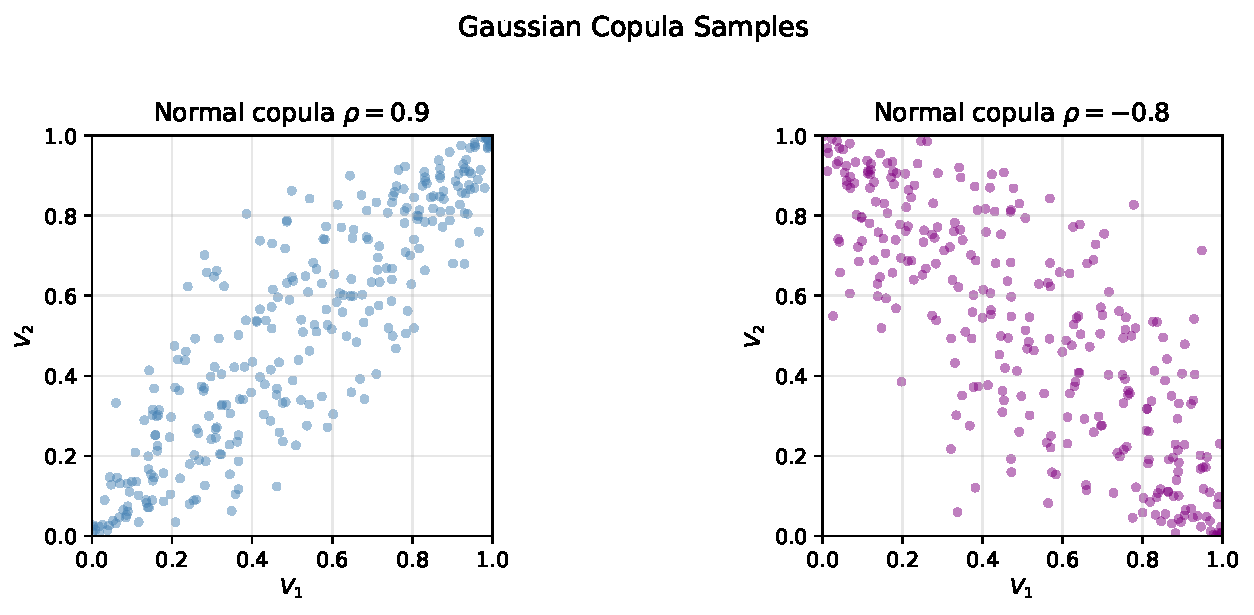
\includegraphics[width=0.60\textwidth]{fig_normal_copula}
  \caption{Gaussian copula samples: $\rho = 0.9$ (left, strong positive dependence,
    most points near the $V_1 = V_2$ diagonal) vs.\ $\rho = -0.8$ (right, strong
    negative dependence, most points near the anti-diagonal $V_1 + V_2 \approx 1$).}
\end{figure}

\framebreak

\begin{alertblock}{Key Insight: Why Copulas Are Useful}
  Copulas provide a \emph{modular} framework for multivariate simulation:
  \begin{itemize}
    \item \textbf{Marginals} are fitted to univariate data (e.g.\ fit an exponential
      to claim arrival times, a Pareto to claim sizes).
    \item \textbf{Dependence} is modelled by a copula fitted to the bivariate rank
      correlation of the data.
    \item Sklar's theorem guarantees the combination is always a valid joint
      distribution.
  \end{itemize}
  This modular approach is widely used in finance (credit risk modelling of multiple
  defaults), insurance (modelling correlated aggregate losses), and environmental
  science (modelling joint extremes such as simultaneous high temperature and
  drought).  The key advantage is that changing the copula does not alter the
  marginal distributions, and vice versa.
\end{alertblock}

\end{frame}

\begin{frame}[fragile]{3.9 Python: Gaussian Copula}
\begin{lstlisting}[style=python, caption={Gaussian copula simulation with arbitrary marginals (Example 3.9.10)}]
import numpy as np
from scipy.stats import norm

rng = np.random.default_rng(42)

def sample_gaussian_copula(rho, n, rng):
    """
    Sample (V1, V2) from the Gaussian copula with correlation rho.
    Step 1: Generate bivariate normal with corr. rho via Cholesky.
    Step 2: Apply normal CDF to each component to get U[0,1] marginals.
    """
    Sigma = np.array([[1.0, rho], [rho, 1.0]])
    A = np.linalg.cholesky(Sigma)   # Sigma = A @ A.T
    Z = rng.standard_normal((2, n))
    W = A @ Z                        # bivariate normal with corr rho
    V1 = norm.cdf(W[0])              # transform to uniform marginals
    V2 = norm.cdf(W[1])
    return V1, V2

def transform_marginals(V1, V2):
    """Transform copula samples (V1, V2) to Exp(1) x Par(1) marginals."""
    X = -np.log(1 - V1)        # F_Exp^{-1}(V1): Exp(1) quantile
    Y = 1.0 / (1 - V2) - 1    # F_Par^{-1}(V2): Par(alpha=1) quantile
    return X, Y

V1, V2 = sample_gaussian_copula(rho=0.8, n=5000, rng=rng)
print(f"Copula Corr(V1,V2) = {np.corrcoef(V1,V2)[0,1]:.3f}  (target rho=0.8)")

X, Y = transform_marginals(V1, V2)
print(f"Exp(1) mean: {X.mean():.3f}  (theory: 1.0)")
# Par(1) has infinite mean; check median instead
print(f"Par(1) median: {np.median(Y):.3f}  (theory: 1.0)")
\end{lstlisting}
\end{frame}

% ============================================================
\section{3.10 Heaviness of Distributions}
% ============================================================

\begin{frame}[allowframebreaks]{3.10 Can We See the ``Heaviness'' of a Distribution?}

The tail behaviour of a distribution has dramatic practical consequences for
Monte Carlo estimation.  We now illustrate this through simulation, comparing
running averages of sequences drawn from several distributions that all have
the \emph{same} theoretical mean $\EE[X_i] = 1$ (where the mean is finite),
but with very different tail behaviours.

\begin{columns}
  \column{0.50\textwidth}
  \begin{block}{Distributions Compared (all with mean $= 1$)}
    \begin{tabular}{@{}lll@{}}
      \toprule
      Distribution & Tail & Variance \\
      \midrule
      $\NN(1,1)$ & Light & 1 \\
      $\mathrm{Exp}(1)$ & Light & 1 \\
      $\mathrm{LN}(-1/2,1)$ & Moderate & $\approx 4.67$ \\
      $\mathrm{W}(1/2,\sqrt{2})$ & Moderate & Finite \\
      $\mathrm{Par}(1.2)$ scaled & Very heavy & $\infty$ \\
      \bottomrule
    \end{tabular}

    Here $\mathrm{LN}(\mu, \sigma)$ is the log-normal with $\log$-parameters $\mu$
    (mu) and $\sigma$ (sigma), and $\mathrm{W}(k, s)$ is the Weibull with shape $k$
    and scale $s$.
  \end{block}

  \column{0.48\textwidth}
  \begin{alertblock}{What to Expect}
    For light-tailed distributions ($\NN$, $\mathrm{Exp}$): the running average
    $S_n/n = (X_1 + \cdots + X_n)/n$ converges smoothly toward the true mean
    of 1, with fluctuations shrinking like $1/\sqrt{n}$ (the CLT rate).

    \medskip
    For $\mathrm{Par}(\alpha)$ with $\alpha \le 2$: the variance is
    \emph{infinite}, so the CLT convergence rate $1/\sqrt{n}$ does not apply.
    Running averages converge far more slowly and show sudden large jumps
    whenever a very large value $X_i$ is drawn.
  \end{alertblock}
\end{columns}

\framebreak

\begin{figure}
  \centering
  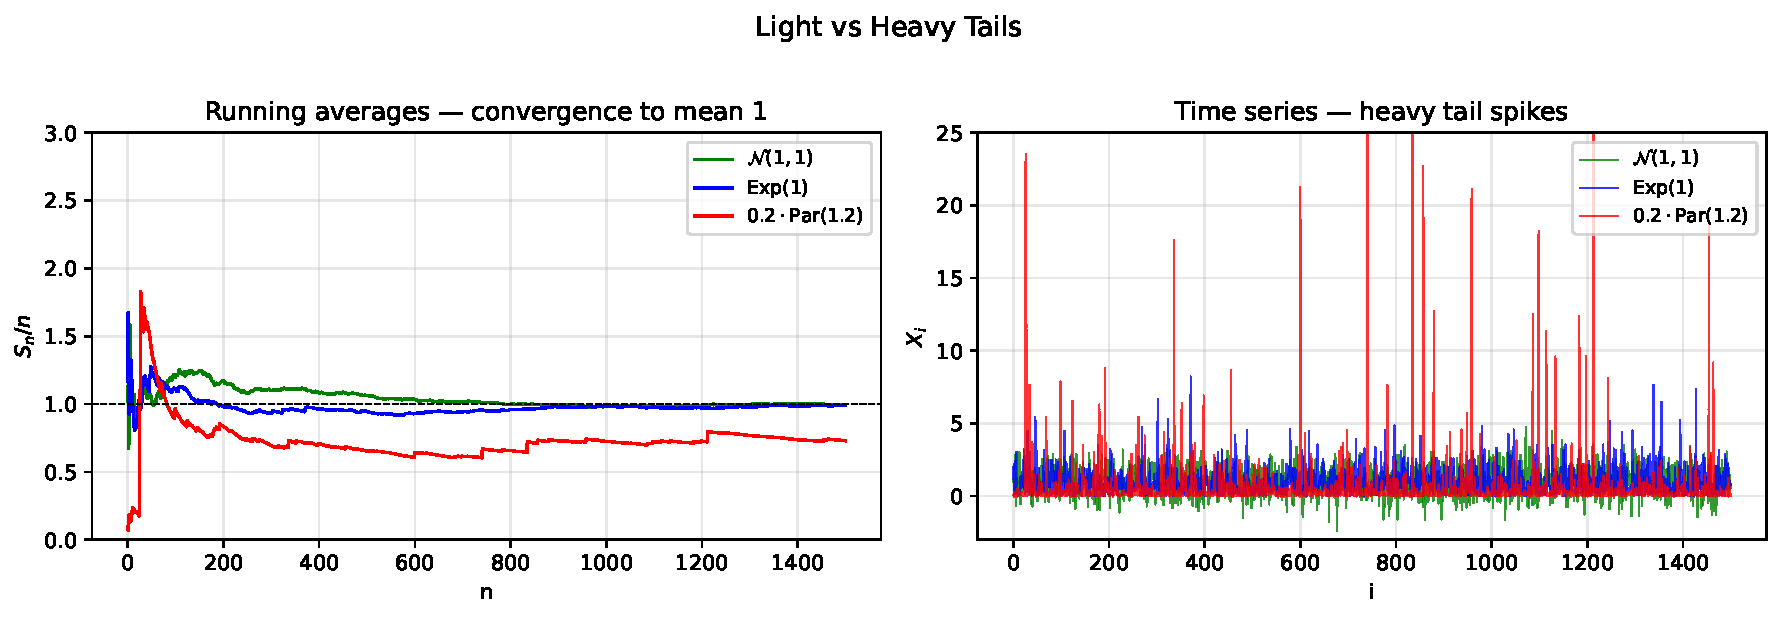
\includegraphics[width=\textwidth]{fig_heavy_tail}
  \caption{(a) Running averages $S_n/n$ for $n = 1, \ldots, 5000$ samples.
    The Normal (blue) and Exp (orange) running averages converge quickly to 1.
    The Pareto($1.2$) (red) shows persistent large fluctuations and sudden
    upward jumps whenever a very large value is drawn.
    (b) The corresponding time series of individual $X_i$ values.  The
    Pareto draws include rare but enormous spikes that dominate the running sum,
    preventing rapid convergence.}
\end{figure}

\framebreak

\begin{block}{QQ Plots for Tail Detection}
  A \emph{quantile-quantile} (QQ) plot compares the \emph{sample quantiles}
  of observed data against the \emph{theoretical quantiles} of a reference
  distribution (usually $\NN(0,1)$ after standardisation).  The procedure:
  sort the data $X_{(1)} \le X_{(2)} \le \cdots \le X_{(n)}$; the $k$-th
  point is $(X_{(k)},\; \Phi^{-1}(k/(n+1)))$.

  \begin{itemize}
    \item \textbf{Light-tailed data:} the QQ plot points lie approximately
      on a straight line through the origin.  This means the sample has
      similar extreme values to what a normal distribution would predict.
    \item \textbf{Heavy-tailed data:} the upper-right corner curves steeply
      upward (the sample has much larger maxima than the normal predicts).
      Similarly, the lower-left corner may curve downward for heavy left tails.
    \item \textbf{Skewed data:} only one tail curves away from the line.
  \end{itemize}
\end{block}

\begin{figure}
  \centering
  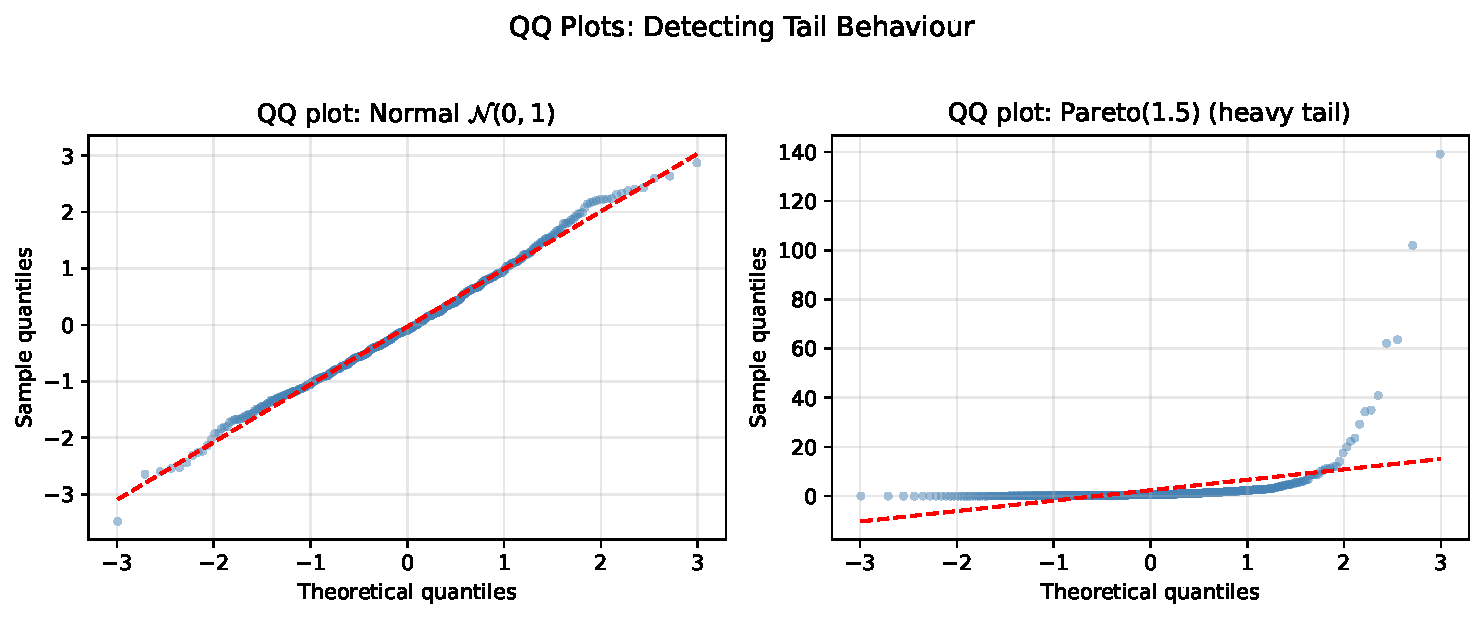
\includegraphics[width=0.68\textwidth]{fig_qq_plots}
  \caption{QQ plots against the $\NN(0,1)$ reference.
    Left: $\NN(0,1)$ data --- the points lie on a straight line, confirming normality.
    Right: $\mathrm{Par}(1.5)$ data --- the upper-right corner curves sharply upward,
    indicating the distribution has a much heavier right tail than normal.}
\end{figure}

\begin{alertblock}{Key Takeaway: Tail Heaviness Is Observable}
  Heavy-tailedness is not just a theoretical property --- it is directly visible
  in simulations.  QQ plots reveal it in the shape of the scatter, and running
  averages reveal it through slow convergence and sudden large jumps.
  In Monte Carlo estimation with heavy-tailed estimators (i.e.\ estimators with
  heavy-tailed distributions), no practical sample size may be large enough
  to give reliable results without variance reduction techniques (Chapter 5).
\end{alertblock}

\end{frame}

% ============================================================
\section{Summary}
% ============================================================

\begin{frame}[allowframebreaks]{Chapter 3 --- Summary of All Methods}

  This chapter has developed a complete toolkit for generating random variables
  from arbitrary distributions, using only uniform random numbers as a primitive.
  The table below gives a concise reference for all methods covered.

  \begin{block}{Complete Method Reference Table}
    \begin{tabular}{@{}llp{4.8cm}@{}}
      \toprule
      Method & Algorithm & Key idea \\
      \midrule
      ITM (general) & 6 & $X = F^{\leftarrow}(U)$; works when $\FInv$ is computable \\
      ITM-Exp & 7 & $X = -\log(U)/\lambda$ \\
      ITM-Par & 8 & $X = U^{-1/\alpha} - 1$ \\
      Geometric closed form & -- & $X = \lfloor\log U/\log p\rfloor$ \\
      ITM-d (discrete) & 9 & Sequential accumulation; $O(\EE Y)$ cost \\
      ITR (ratio recursion) & 10 & Ratio $c_{k+1} = p_{k+1}/p_k$; $(a,b,0)$ class \\
      DB (direct binomial) & 11 & Sum $n$ Bernoulli trials; $O(n)$ cost \\
      Erlang sum & -- & $X = -\log(\prod U_i)/\lambda$; stable via log-sum \\
      DP (Poisson via renewal) & 12 & Count Exp(1) inter-arrivals; $O(\lambda)$ cost \\
      AR-d & 14 & $p_j \le cq_j$; accept with probability $p_j/(cq_j)$ \\
      AR-c & 16 & $f \le cg$; accept with probability $f(Y)/(cg(Y))$ \\
      AR-N (half-normal) & 17 & Exp(1) proposal; $c = \sqrt{2e/\pi}$; $76\%$ accept \\
      Composition & -- & Sample component $J \sim (p_j)$, draw from $g_J$ \\
      Box-Muller & 20 & Polar transform; two normals from two uniforms \\
      Marsaglia-Bray & 21 & Polar in disc; avoids trig; $78.5\%$ accept \\
      ITM normal (BSM) & 22 & Rational approx for $\Phi^{-1}$; vectorizable \\
      Cholesky (multivariate) & -- & $\mathbf{X} = \mathbf{A}\mathbf{Z} + \boldsymbol{\mu}$; $\mathbf{A}\mathbf{A}^T = \boldsymbol{\Sigma}$ \\
      Normal trick (sphere) & -- & $\mathbf{X} = \mathbf{Z}/\|\mathbf{Z}\| \sim \UU(S_{d-1})$ \\
      Scaled sphere (ball) & -- & $\mathbf{X} = U^{1/d}\mathbf{Z}/\|\mathbf{Z}\| \sim \UU(B_d)$ \\
      Ellipsoid & 23 & Linear transform of $\UU(B_d)$ via Cholesky \\
      Conditional ITM & -- & Marginal first, then conditional \\
      Gaussian copula & -- & Bivariate normal $\to$ $\Phi$ transform; any marginals \\
      \bottomrule
    \end{tabular}
  \end{block}

\framebreak

  \begin{columns}
    \column{0.50\textwidth}
    \begin{block}{Key Formulas at a Glance}
      \begin{align*}
        \text{ITM: } & X = F^{\leftarrow}(U) \\[3pt]
        \text{Exp: } & X = -\tfrac{1}{\lambda}\log U \\[3pt]
        \text{Par: } & X = U^{-1/\alpha} - 1 \\[3pt]
        \text{Geo: } & X = \lfloor \tfrac{\log U}{\log p}\rfloor \\[3pt]
        \text{Erlang: } & X = -\tfrac{\log(\prod U_i)}{\lambda} \\[3pt]
        \text{BM: } & Z = \sqrt{-2\log U_1}\cos(2\pi U_2) \\[3pt]
        \text{MVN: } & \mathbf{X} = \mathbf{A}\mathbf{Z} + \boldsymbol{\mu} \\[3pt]
        \text{Sphere: } & \mathbf{X} = \mathbf{Z}/\|\mathbf{Z}\| \\[3pt]
        \text{Ball: } & \mathbf{X} = U^{1/d}\mathbf{Z}/\|\mathbf{Z}\|
      \end{align*}
    \end{block}

    \column{0.48\textwidth}
    \begin{block}{Design Principles}
      \begin{itemize}
        \item \textbf{AR method:} choose $c = \sup f(x)/g(x)$ as small as
              possible; smaller $c$ means higher acceptance rate $1/c$ and
              fewer wasted samples.
        \item \textbf{Composition:} use when the target density is a finite or
              infinite mixture of densities that are individually easy to sample.
        \item \textbf{Unknown normalising constants:} AR-c works with
              unnormalised densities $f^*$ and $g^*$ directly.
        \item \textbf{Copulas:} Sklar's theorem separates dependence from
              marginals; fit each independently to data.
        \item \textbf{High-dimensional sphere:} always use the Normal trick;
              rejection from a bounding cube is exponentially inefficient.
        \item \textbf{QQ plots:} use as a visual diagnostic for tail heaviness
              before committing to a Monte Carlo estimator.
      \end{itemize}
    \end{block}
  \end{columns}

\end{frame}

% ============================================================
\section*{References}
% ============================================================

\begin{frame}{3.11 Bibliographical Notes}
  \begin{itemize}
    \item \textbf{Devroye (1986)} --- \textit{Non-Uniform Random Variate Generation}.
          The definitive reference for all methods in this chapter, with
          detailed proofs and efficiency analyses.
    \item \textbf{Knuth (1997)} --- \textit{The Art of Computer Programming, Vol.\ 2}.
          Classical treatment of the inverse transform and discrete methods.
    \item \textbf{Glasserman (2004)} --- \textit{Monte Carlo Methods in Financial Engineering}.
          Covers ITM for normal variables and the Beasley-Springer-Moro algorithm.
    \item \textbf{Asmussen \& Glynn (2007)} --- Simulation Algorithms for Stochastic Systems.
          Fr\'{e}chet-Hoeffding bounds and copulas.
    \item \textbf{Box \& Muller (1958)} --- Original paper introducing Algorithm 20.
    \item \textbf{Marsaglia \& Bray (1964)} --- Original paper introducing Algorithm 21.
    \item \textbf{Madras (2002)} --- AR-c method for Gamma distributions.
    \item \textbf{Wichura (1988), AS241} --- Algorithm underlying \texttt{scipy.stats.norm.ppf}.
    \item \textbf{Embrechts \& Hofert} --- Properties of copulas and generalized inverses.
    \item \textbf{Dagpunar (2007)} --- Composition method, atomic physics example.
    \item \textbf{Ross (2006)} --- Elementary introduction to simulation methods.
  \end{itemize}
\end{frame}

\end{document}
